\documentclass[10pt,aspectratio=169]{beamer}

\usetheme{Madrid}
\usecolortheme{seahorse}
\setbeamertemplate{navigation symbols}{}
\setbeamertemplate{footline}[frame number]

\usepackage[utf8]{inputenc}
\usepackage{graphicx}
\usepackage{booktabs}
\usepackage{tikz}
\usetikzlibrary{arrows.meta,positioning,shapes.geometric}
\usepackage{enumitem}
\setlist[itemize,1]{itemsep=1pt,topsep=1pt,parsep=0pt,partopsep=0pt,leftmargin=1.6em,label=\usebeamertemplate{itemize item}}
\setlist[itemize,2]{itemsep=1pt,topsep=1pt,parsep=0pt,partopsep=0pt,leftmargin=1.4em,label=\usebeamertemplate{itemize subitem}}
\setbeamerfont{itemize/enumerate body}{size=\footnotesize}
\setbeamerfont{itemize/enumerate subbody}{size=\scriptsize}
\setbeamerfont{frametitle}{size=\large}
\usepackage{hyperref}
\hypersetup{colorlinks=true,linkcolor=,urlcolor=blue,citecolor=blue}

% Figures: report/05_figs.Rmd (fig1--6 and fig_mac_*).
\graphicspath{{./}}

\title[BIM Resilience: Biological Simulations]{Biological Simulations: Stocks, Advice, and Forecast}
\subtitle{Advice \& scenarios from the Biological Model, and how CREST turns them into an industry resilience tool}
\author{Laurence T. Kell}
\institute{BIM Resilience Project}
\date{\today}

\begin{document}

\begin{frame}
  \titlepage
\end{frame}

% ------------------------------------------------------------
\section{Advice \& Trends}

\begin{frame}{1. Advice --- updates, conditioned on the past}
  \begin{columns}[T]
    \begin{column}{0.46\textwidth}
      \footnotesize
      \textbf{Advice is provided} each year either by an
      \vspace{2mm}
      \begin{itemize}
        \item \textbf{\textit{Update}}: add last year's catches and surveys, and re-run the model
        \item Same structure, data and reference points; the time series is extended one year
        \item Figure: successive update peels --- shape is stable, terminal year moves
      \end{itemize}
    \end{column}
    \begin{column}{0.5\textwidth}
      \centering
      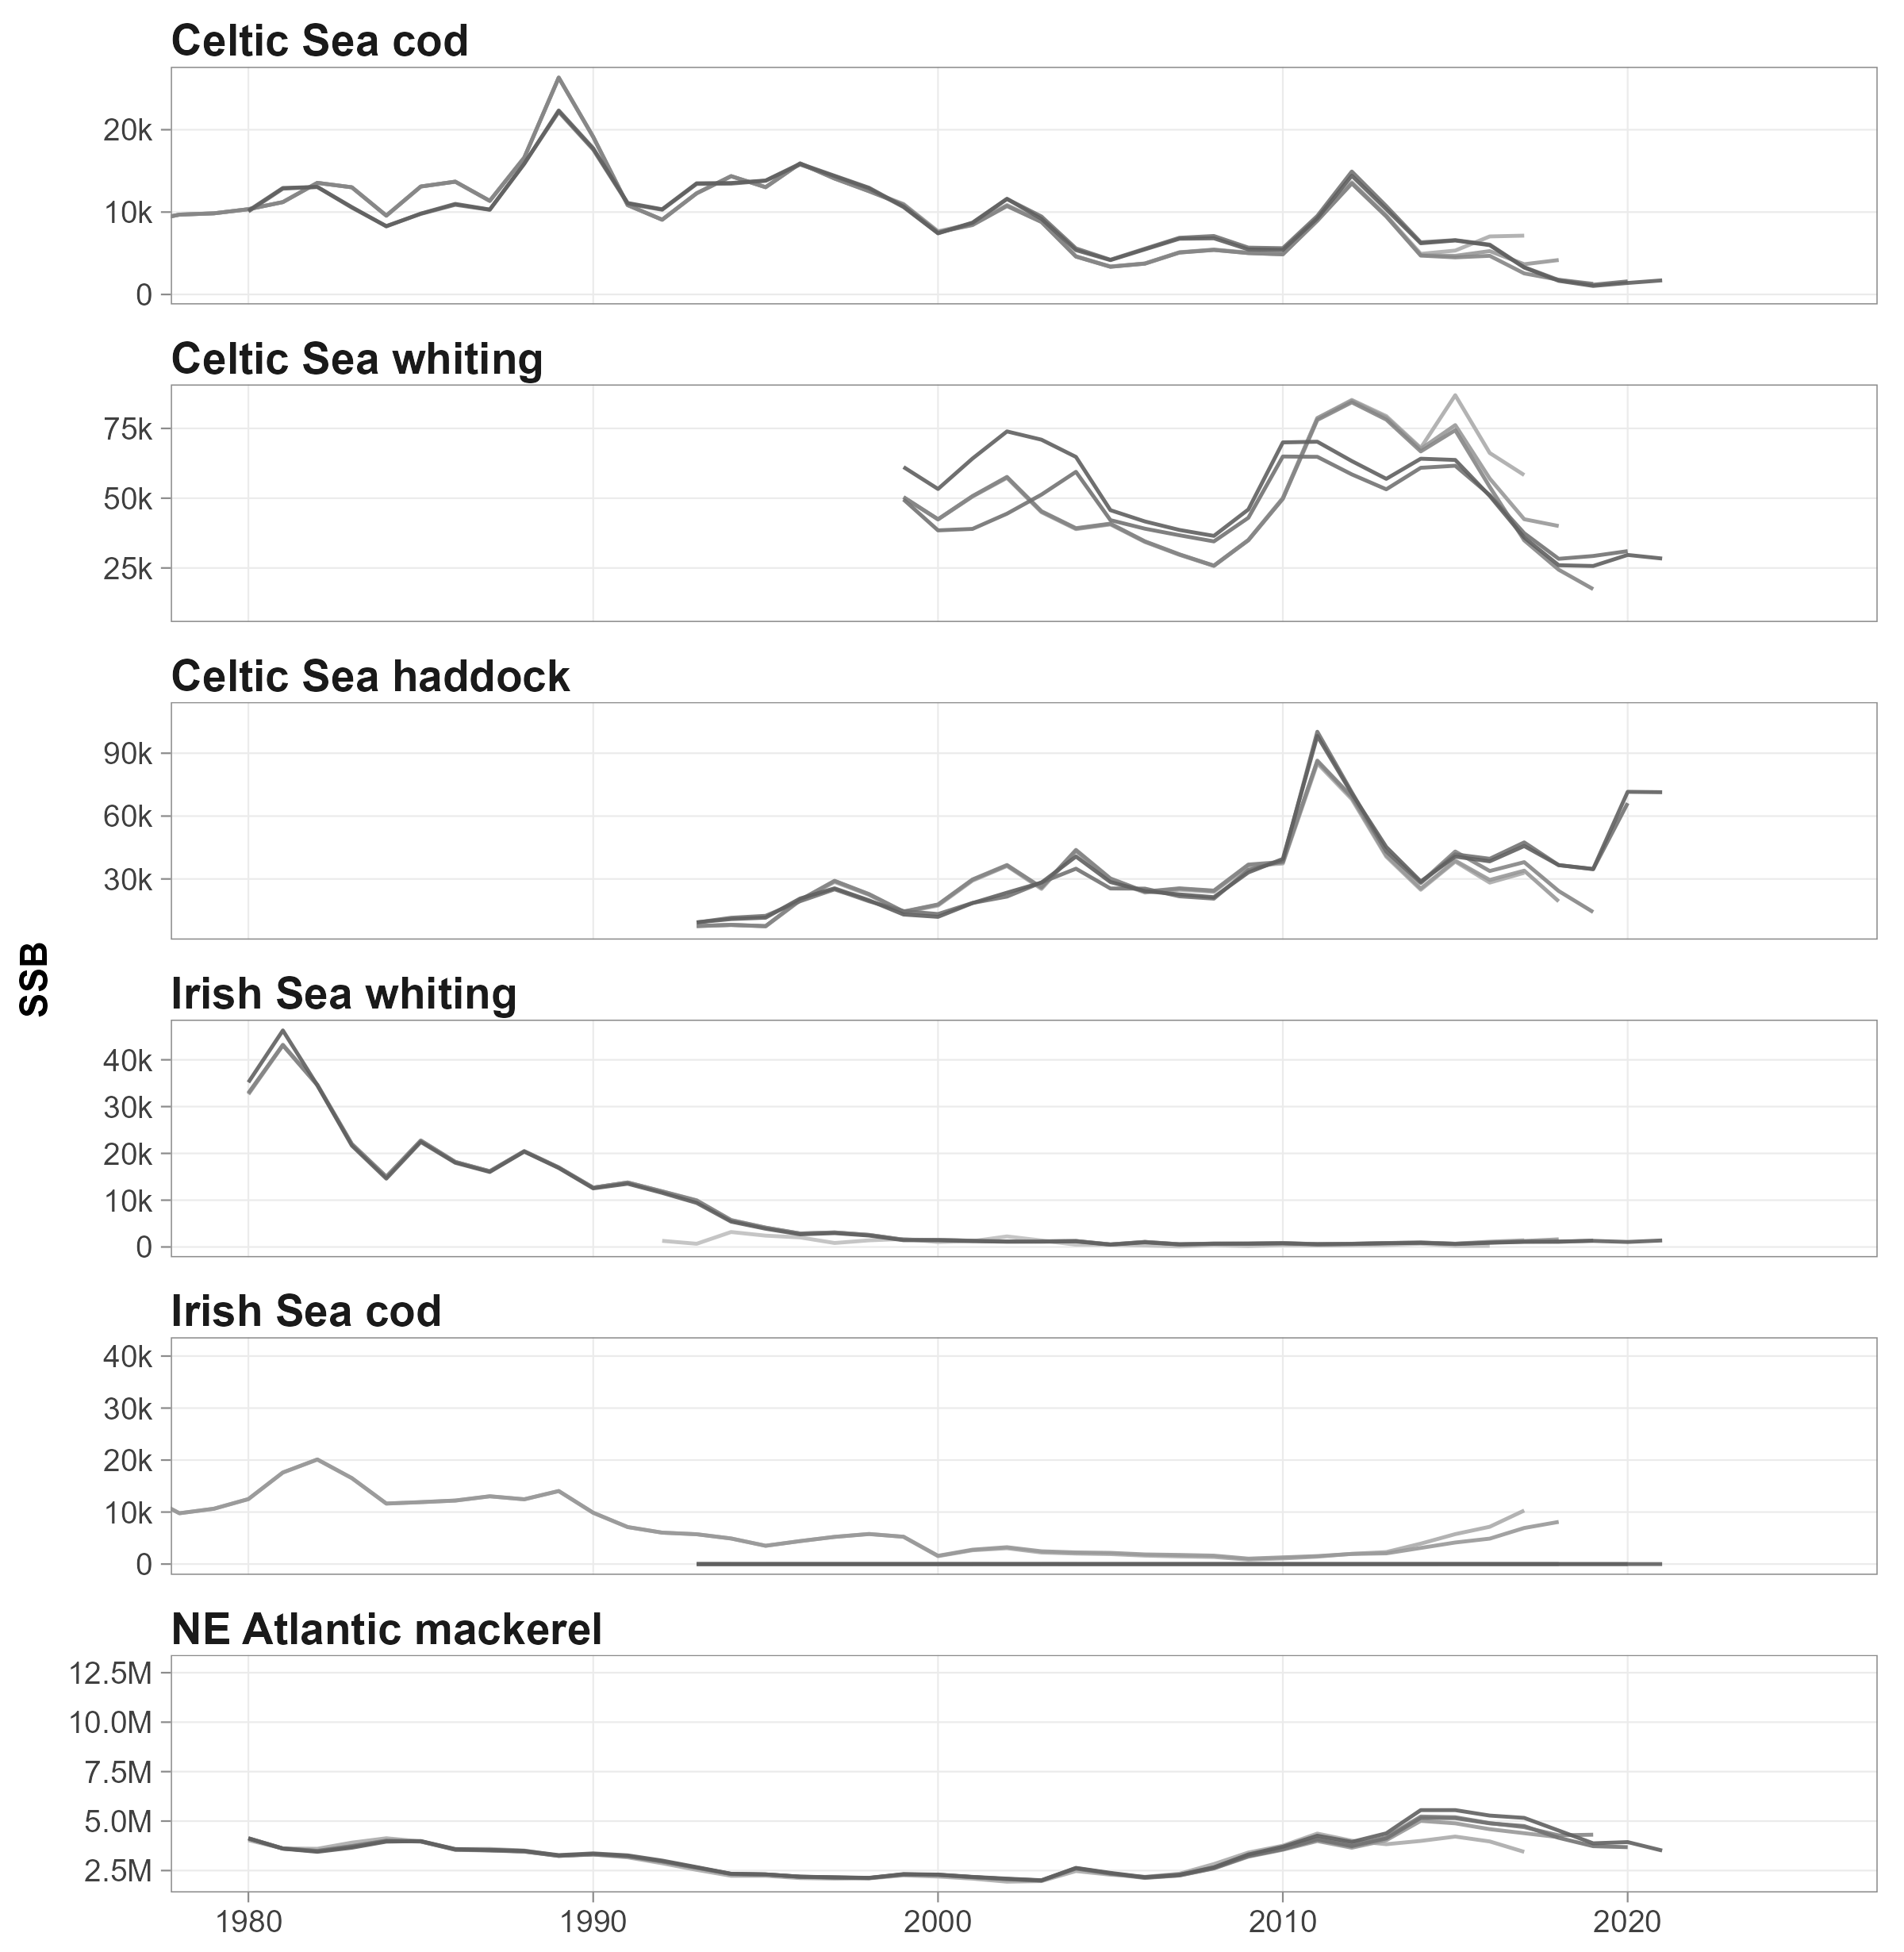
\includegraphics[width=\linewidth]{fig1.png}\\
      {\scriptsize SSB by stock; update peels 2016--2021}
    \end{column}
  \end{columns}
\end{frame}

\begin{frame}{1. Advice --- benchmarks can tell a different story}
  \begin{columns}[T]
    \begin{column}{0.46\textwidth}
      \footnotesize
      \textbf{Advice is provided} each year either by an
      \vspace{2mm}
      \begin{itemize}
        \item \textbf{\textit{Update}}: adding last year's catches and surveys, and re-running the model
        \item \textbf{Benchmark}: full peer-reviewed reset of assumptions, data and reference points; can tell a different story
          \begin{itemize}
            \item Reference points are not fixed: $B_{\mathrm{trigger}}$, $B_{\mathrm{lim}}$, $F_{\mathrm{MSY}}$ shift at a benchmark
            \item Productivity regimes change them further
          \end{itemize}
        \item \textbf{\textit{Take-away}}: reference points and stock status may differ after the next benchmark --- \emph{resilience} means being ready for that
      \end{itemize}
    \end{column}
    \begin{column}{0.5\textwidth}
      \centering
      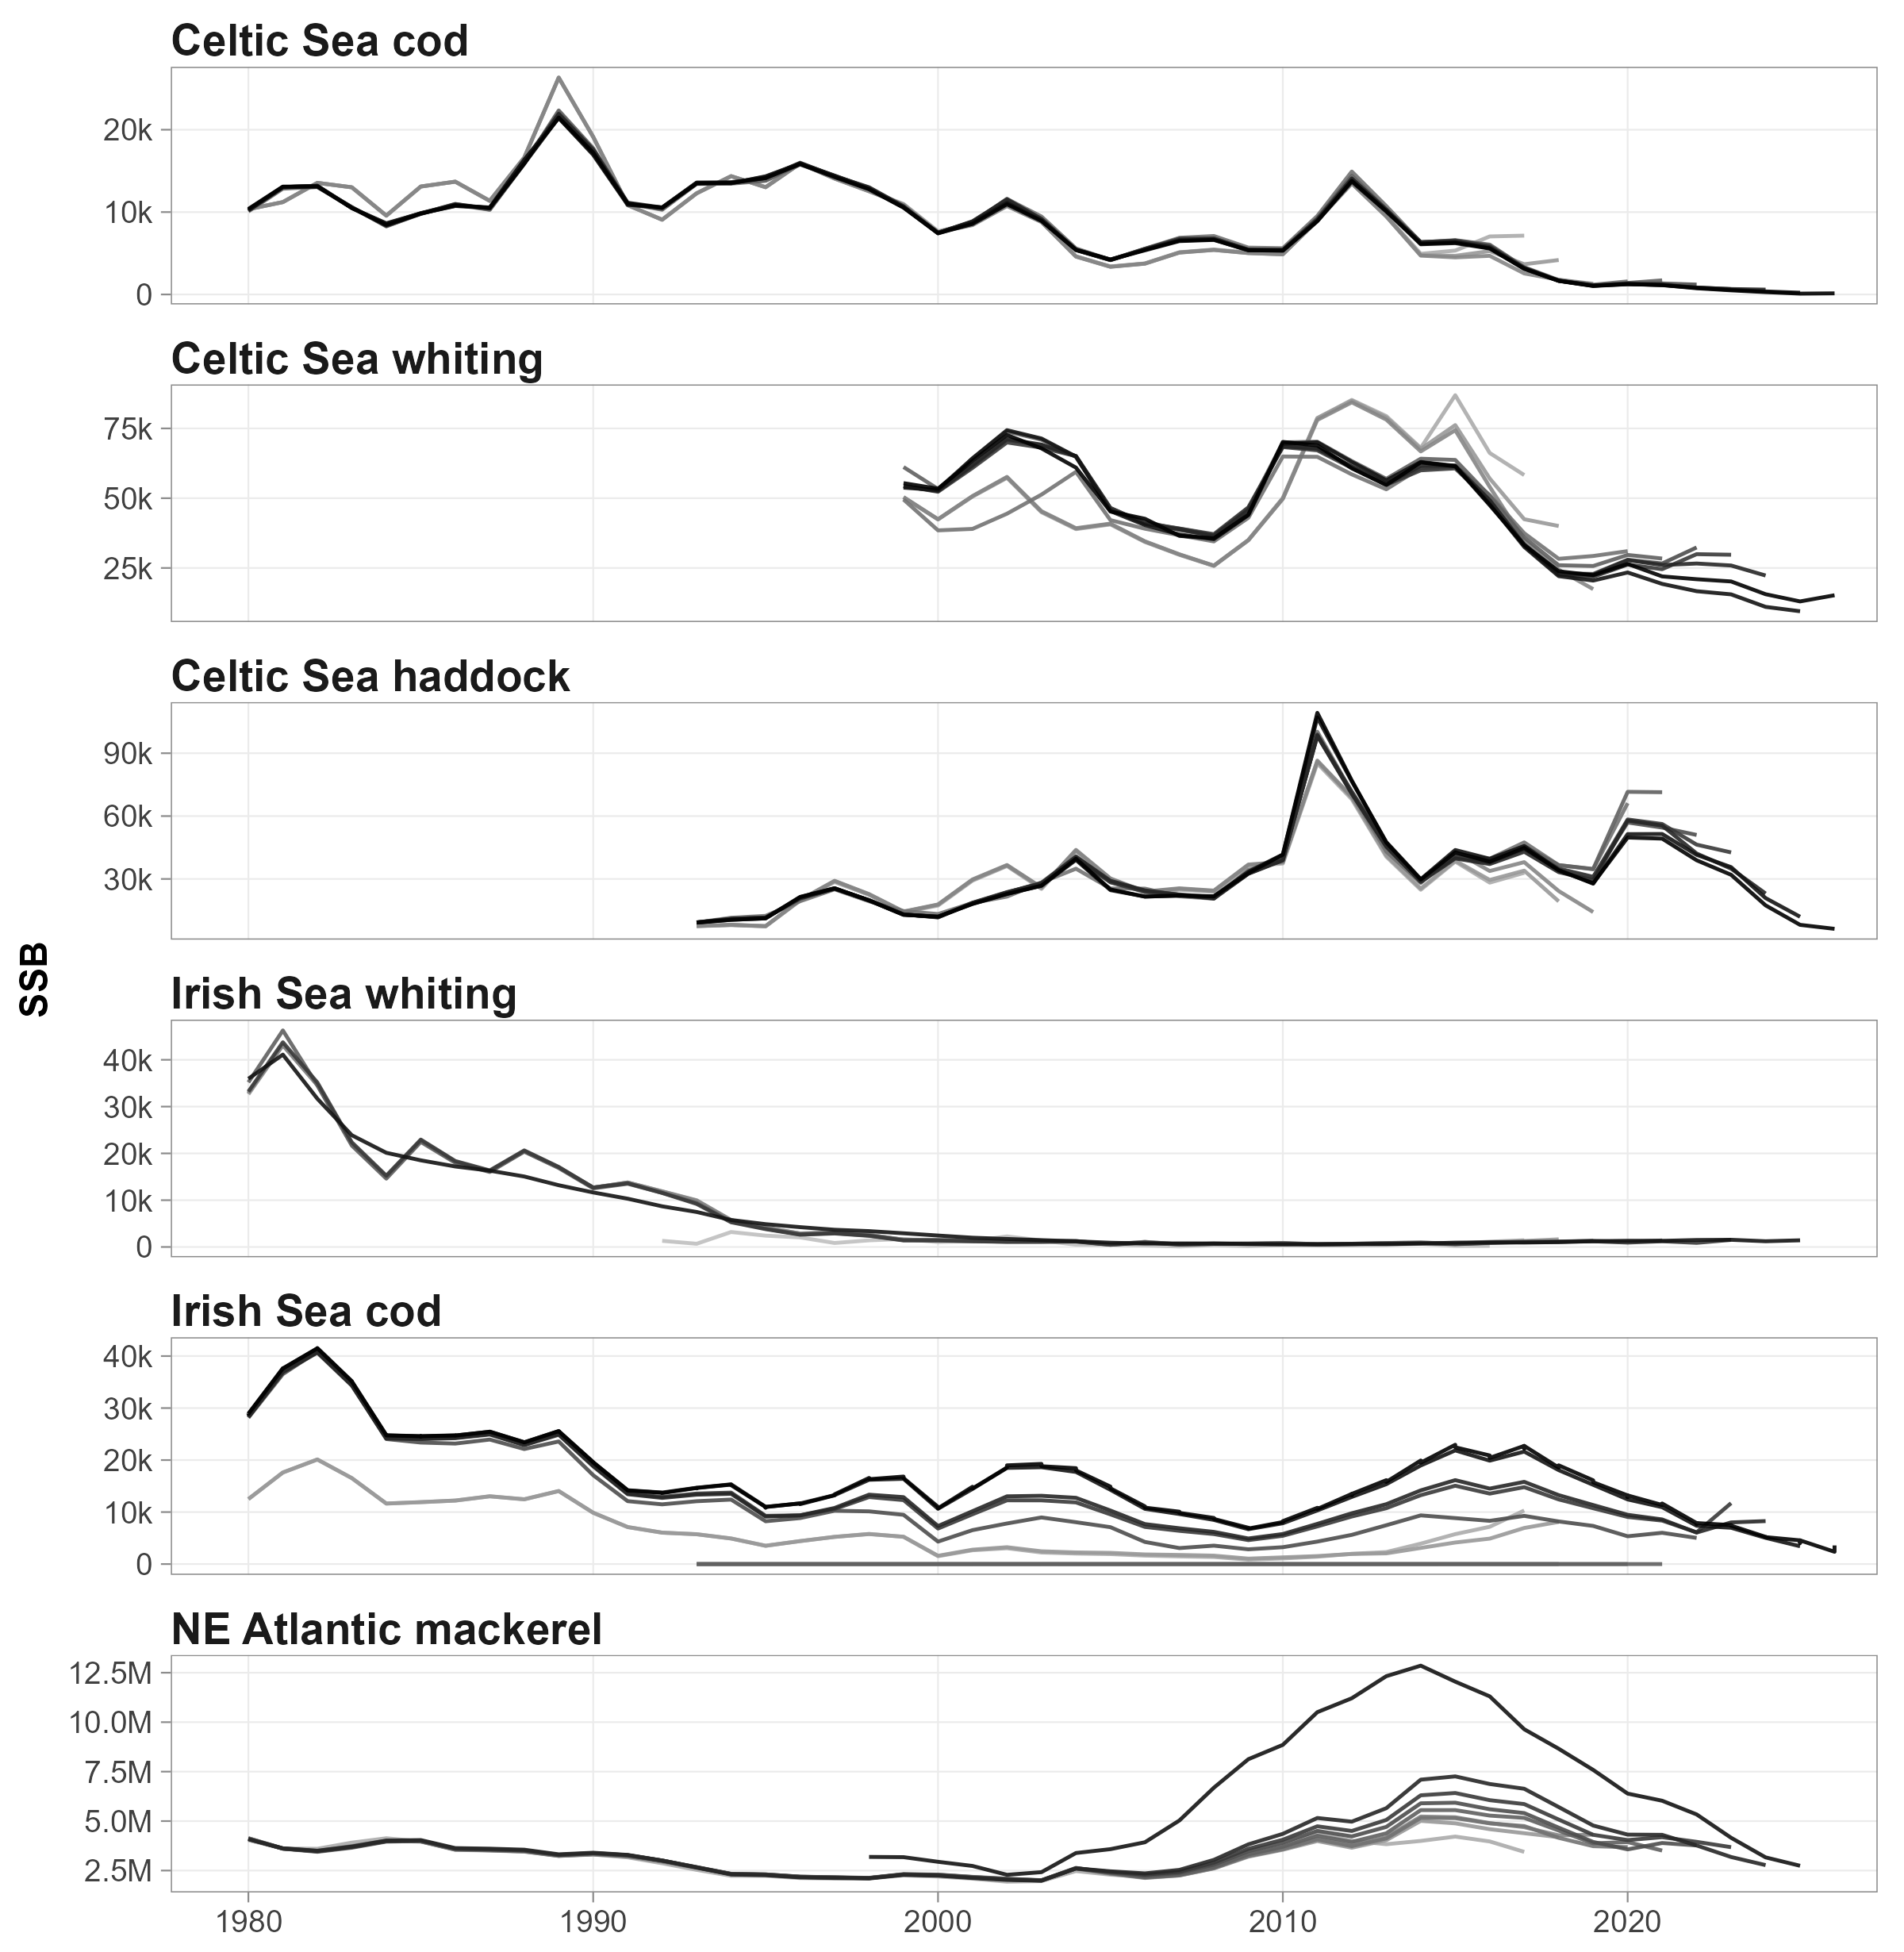
\includegraphics[width=\linewidth]{fig2.png}\\
      {\scriptsize SSB by stock; assessment years 2016--2026}
    \end{column}
  \end{columns}
\end{frame}

\begin{frame}{1. Advice --- status relative to $B_{\mathrm{trigger}}$}
  \begin{columns}[T]
    \begin{column}{0.46\textwidth}
      \footnotesize
      \begin{itemize}
        \item Absolute SSB hides the management scale: what matters for advice is position relative to reference points
        \item Plot: $\mathrm{SSB}/B_{\mathrm{trigger}}$ (MSY $B_{\mathrm{trigger}}$); red line at 1
        \item Peels that cross the line are the years when status --- and therefore advice narrative --- flips
        \item \textbf{\textit{Take-away}}: a benchmark that moves $B_{\mathrm{trigger}}$ can reclassify the same biomass history
      \end{itemize}
    \end{column}
    \begin{column}{0.5\textwidth}
      \centering
      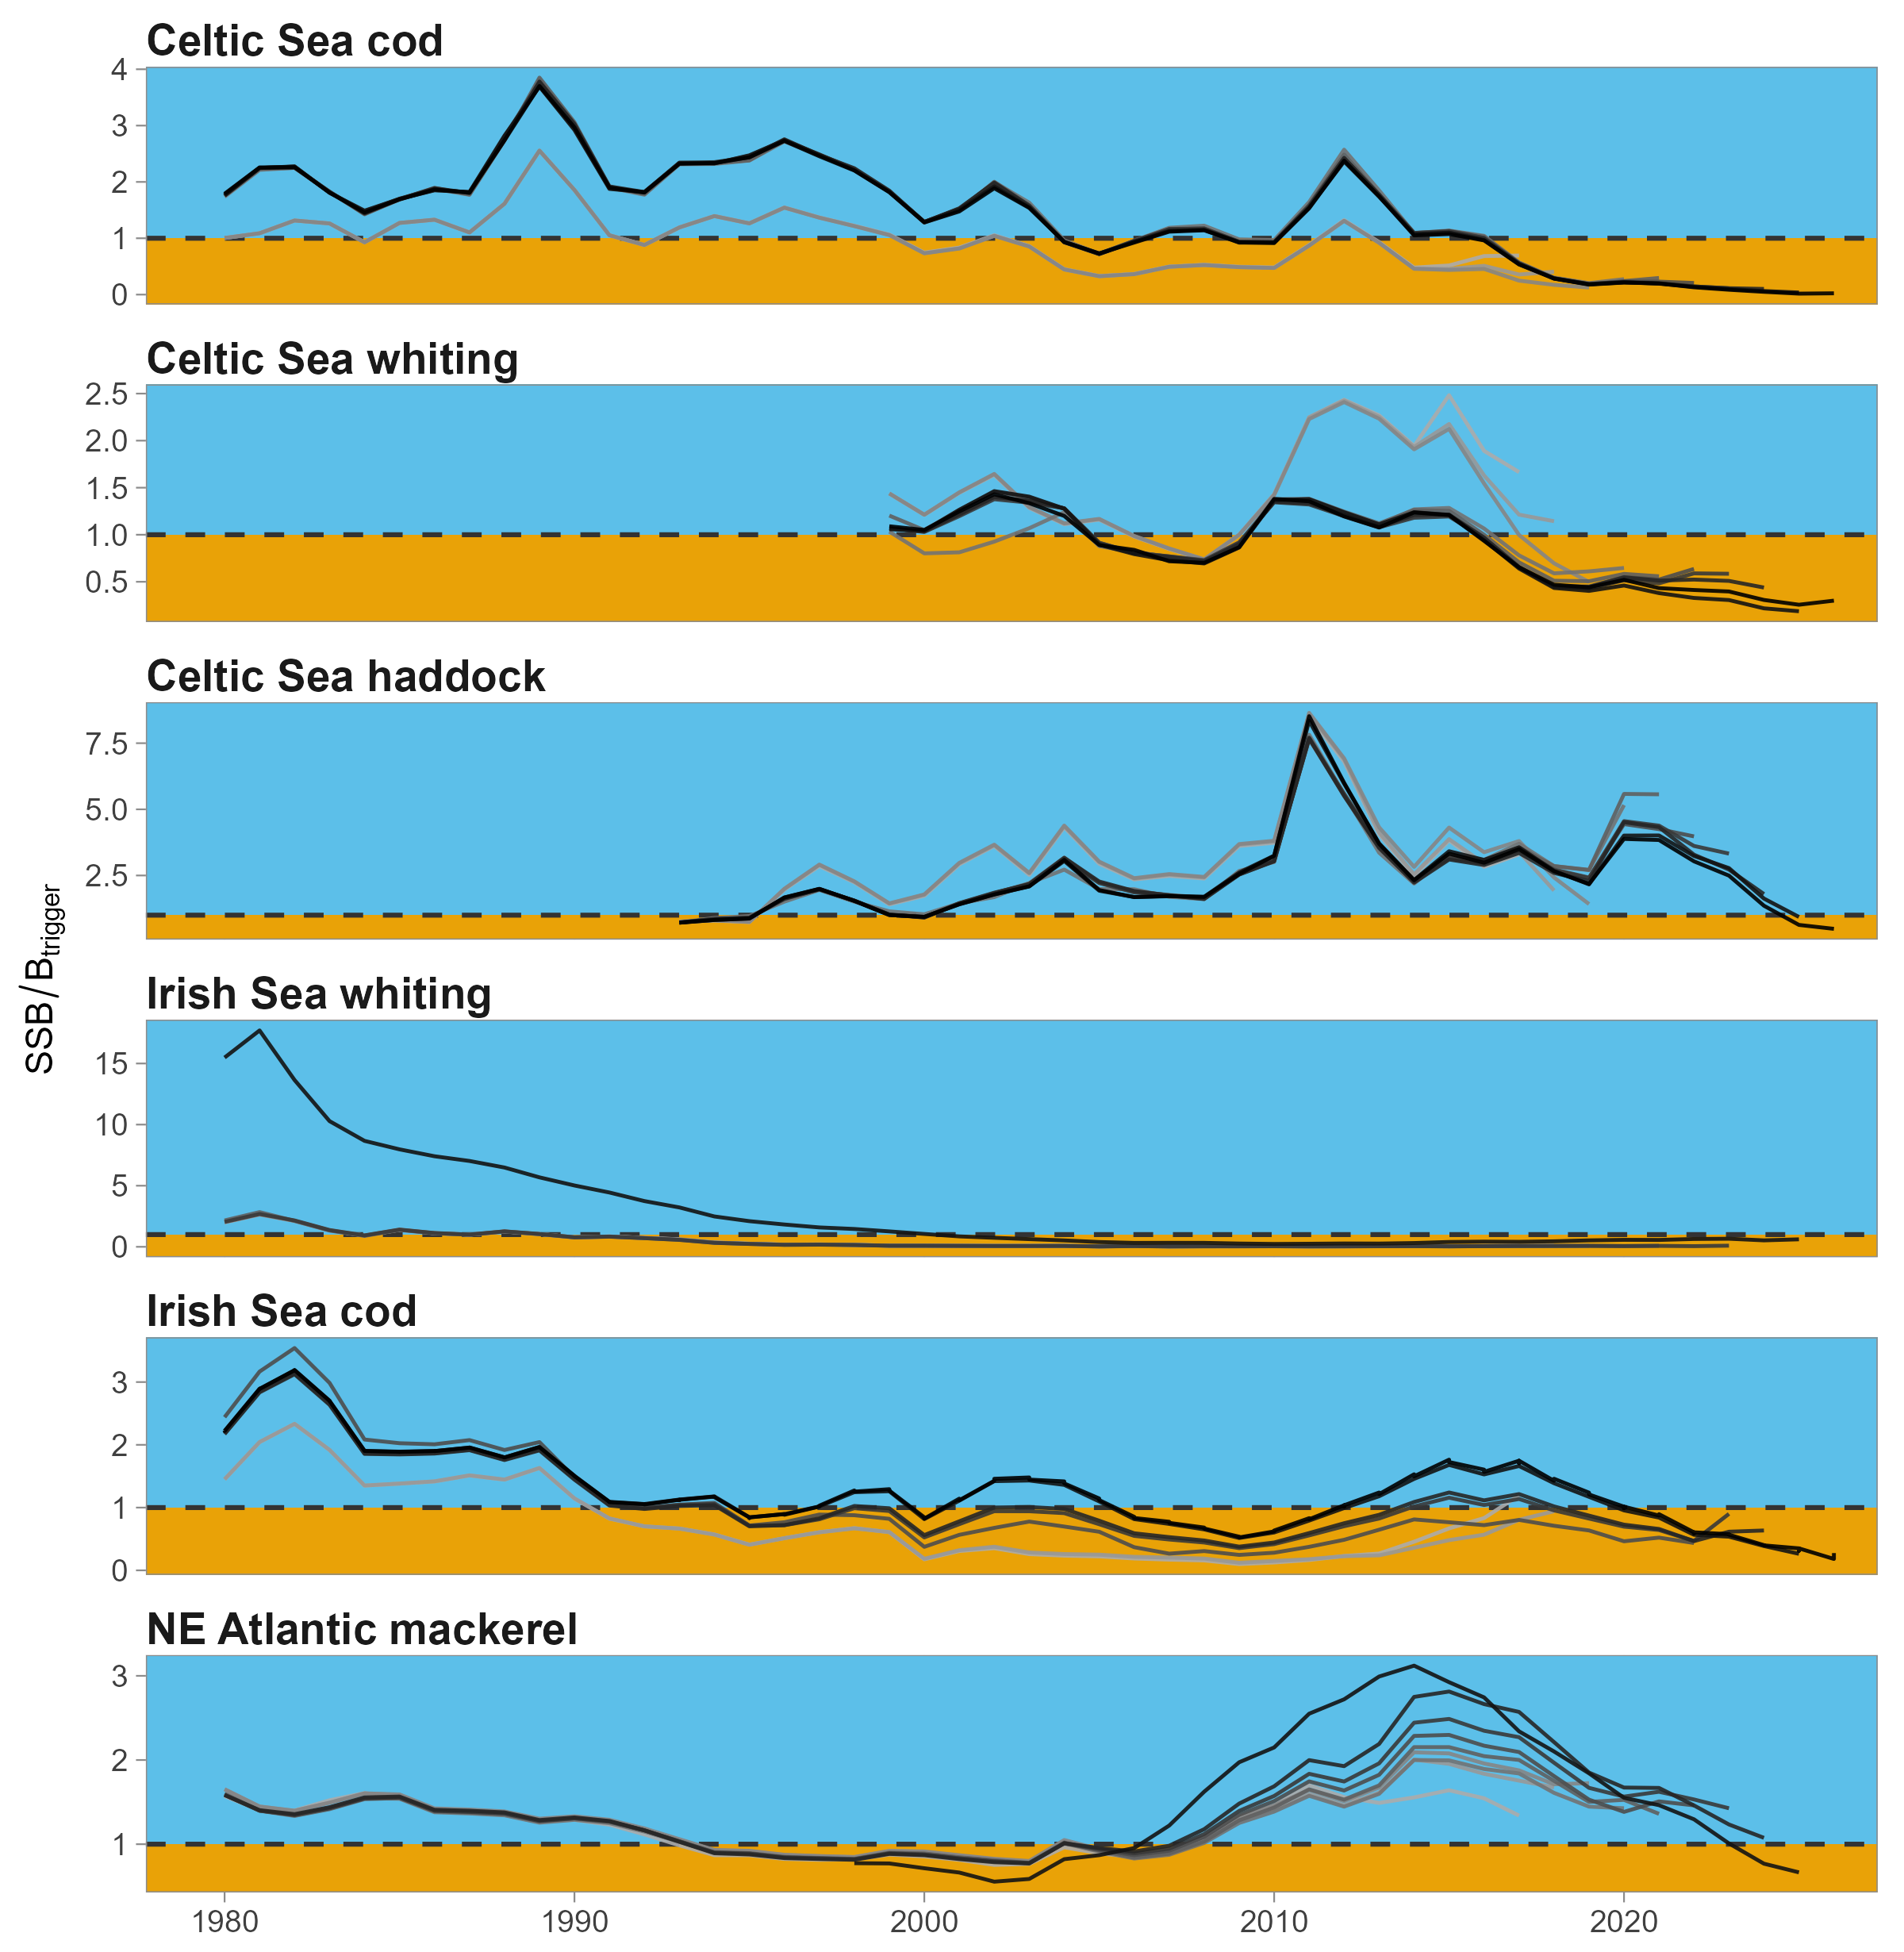
\includegraphics[width=\linewidth]{fig3.png}\\
      {\scriptsize $\mathrm{SSB}/B_{\mathrm{trigger}}$; assessment years 2016--2026}
    \end{column}
  \end{columns}
\end{frame}

% ------------------------------------------------------------
\section{Scenarios}

\begin{frame}{2. Scenarios --- pelagics}
  \begin{columns}[T]
    \begin{column}{0.46\textwidth}
      \footnotesize
      \begin{itemize}
        \item \textbf{Pelagics}: boarfish, western horse mackerel, NEA mackerel, blue whiting
        \item Shared ``what ifs'' under fixed $F$ / recruitment assumptions:
          \begin{itemize}
            \item Status-quo $F$ (recent mean)
            \item Status-quo $F$ with poorer recruitment ($75\%$, $50\%$)
            \item $F_{\mathrm{MSY}}$; and $F_{\mathrm{MSY}}$ under the latest recruitment \emph{regime}
          \end{itemize}
        \item Compare paths \emph{within} a stock: the vertical gap is the assumption that changed
      \end{itemize}
    \end{column}
    \begin{column}{0.5\textwidth}
      \centering
      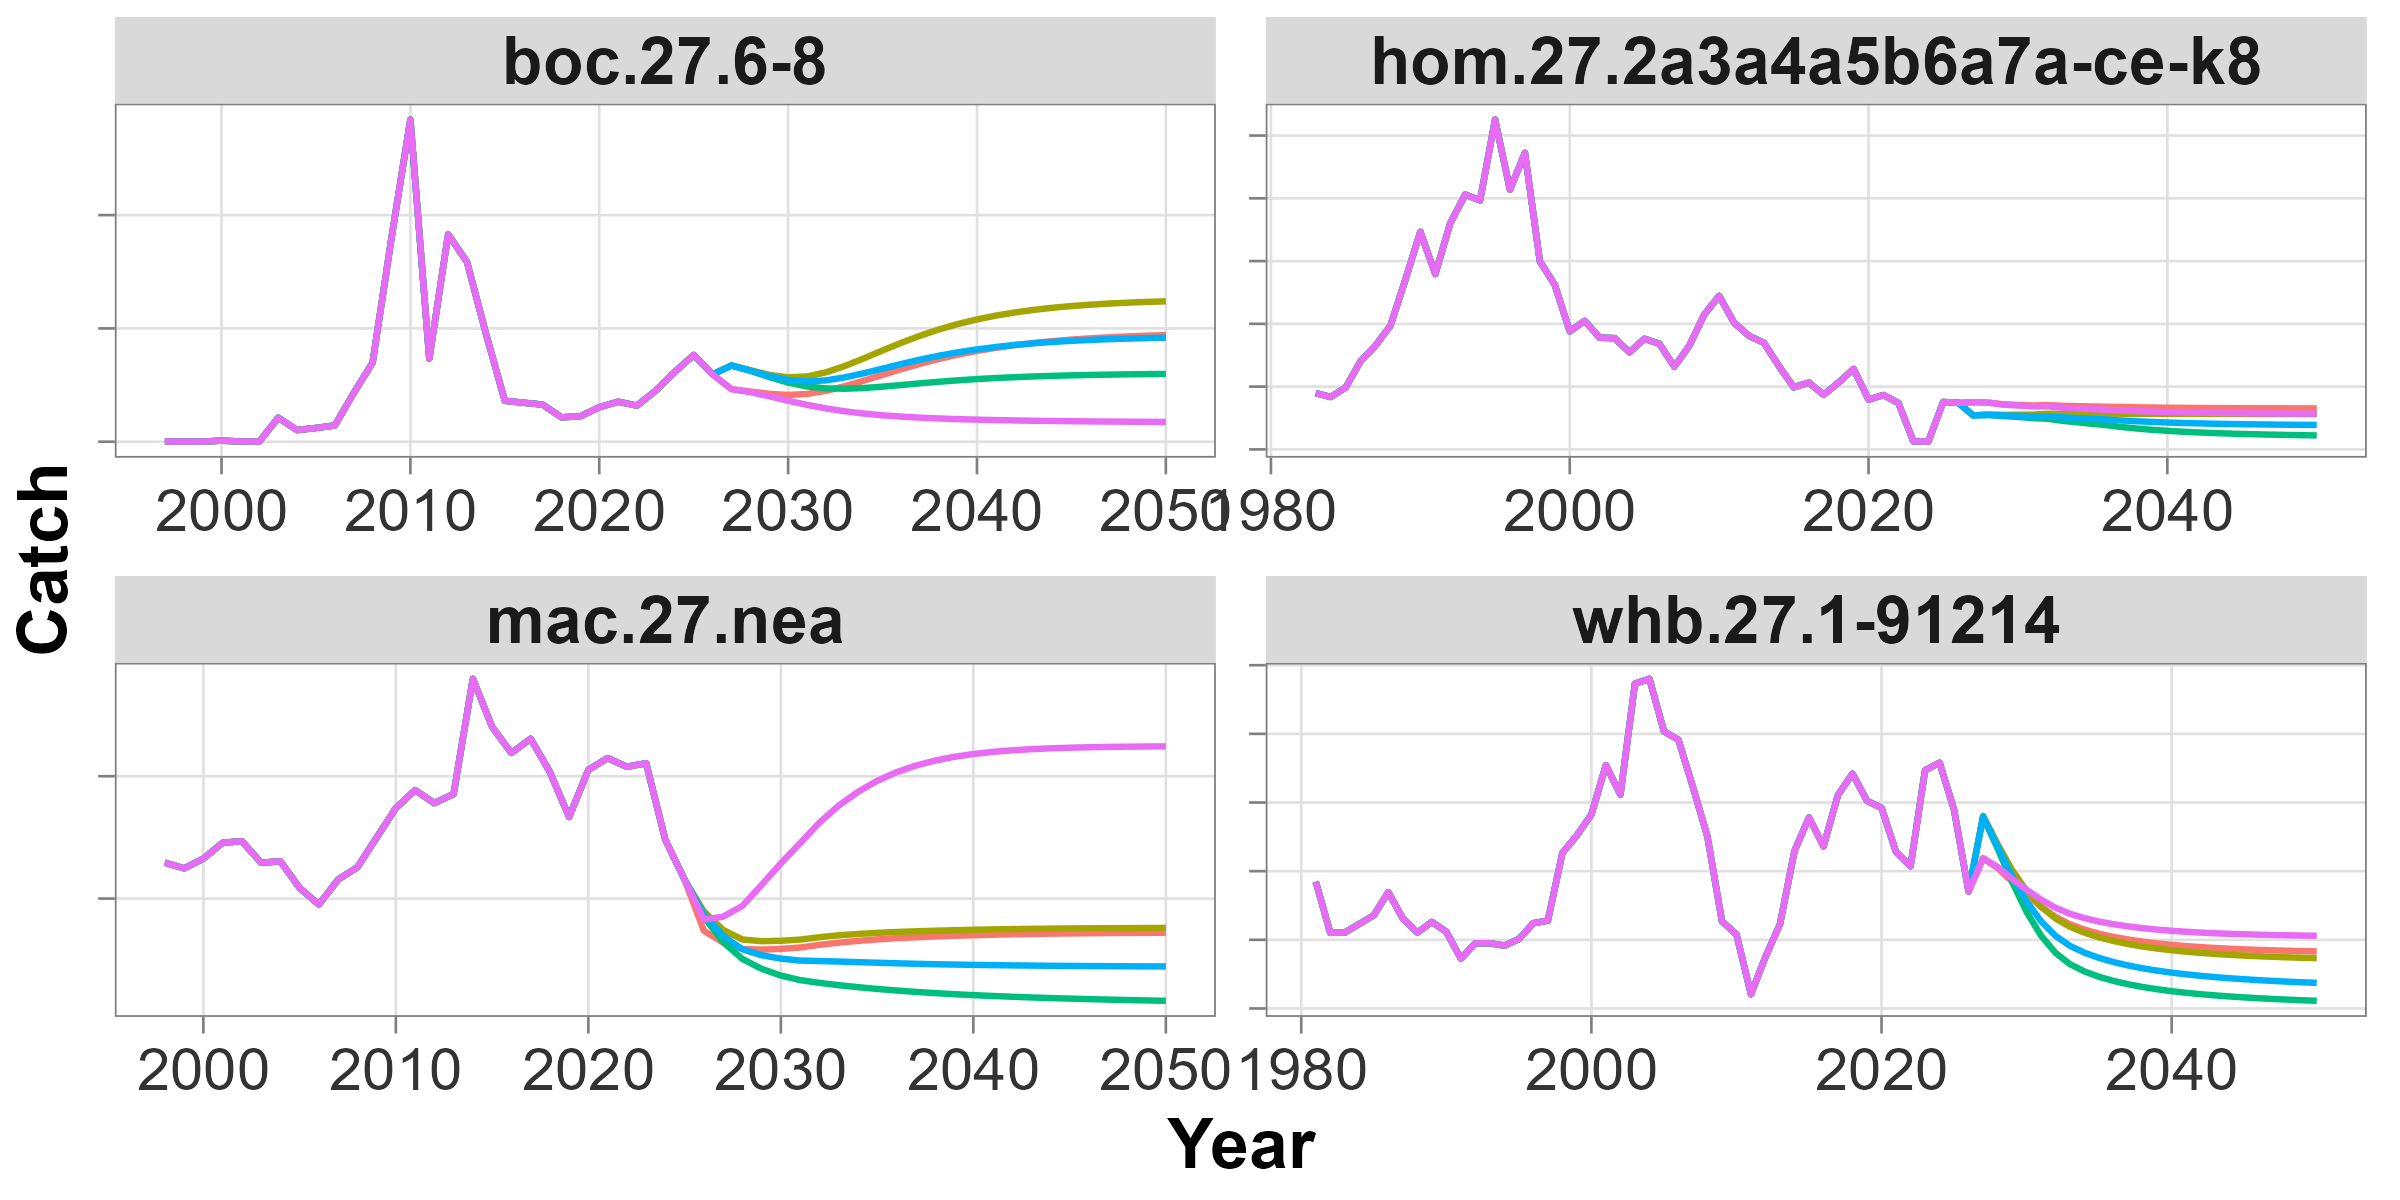
\includegraphics[width=\linewidth]{fig4.png}\\
      {\scriptsize Projected catch by scenario}
    \end{column}
  \end{columns}
\end{frame}

\begin{frame}{2. Scenarios --- demersal}
  \begin{columns}[T]
    \begin{column}{0.46\textwidth}
      \footnotesize
      \begin{itemize}
        \item \textbf{Demersal}: anglerfishes, northern hake, megrims, whitings (west / northern shelf)
        \item Same control table as pelagics: status-quo $F$, reduced recruitment, $F_{\mathrm{MSY}}$, Regime
        \item Resilience reading: does poorer productivity erode catch under current fishing intensity?
      \end{itemize}
    \end{column}
    \begin{column}{0.5\textwidth}
      \centering
      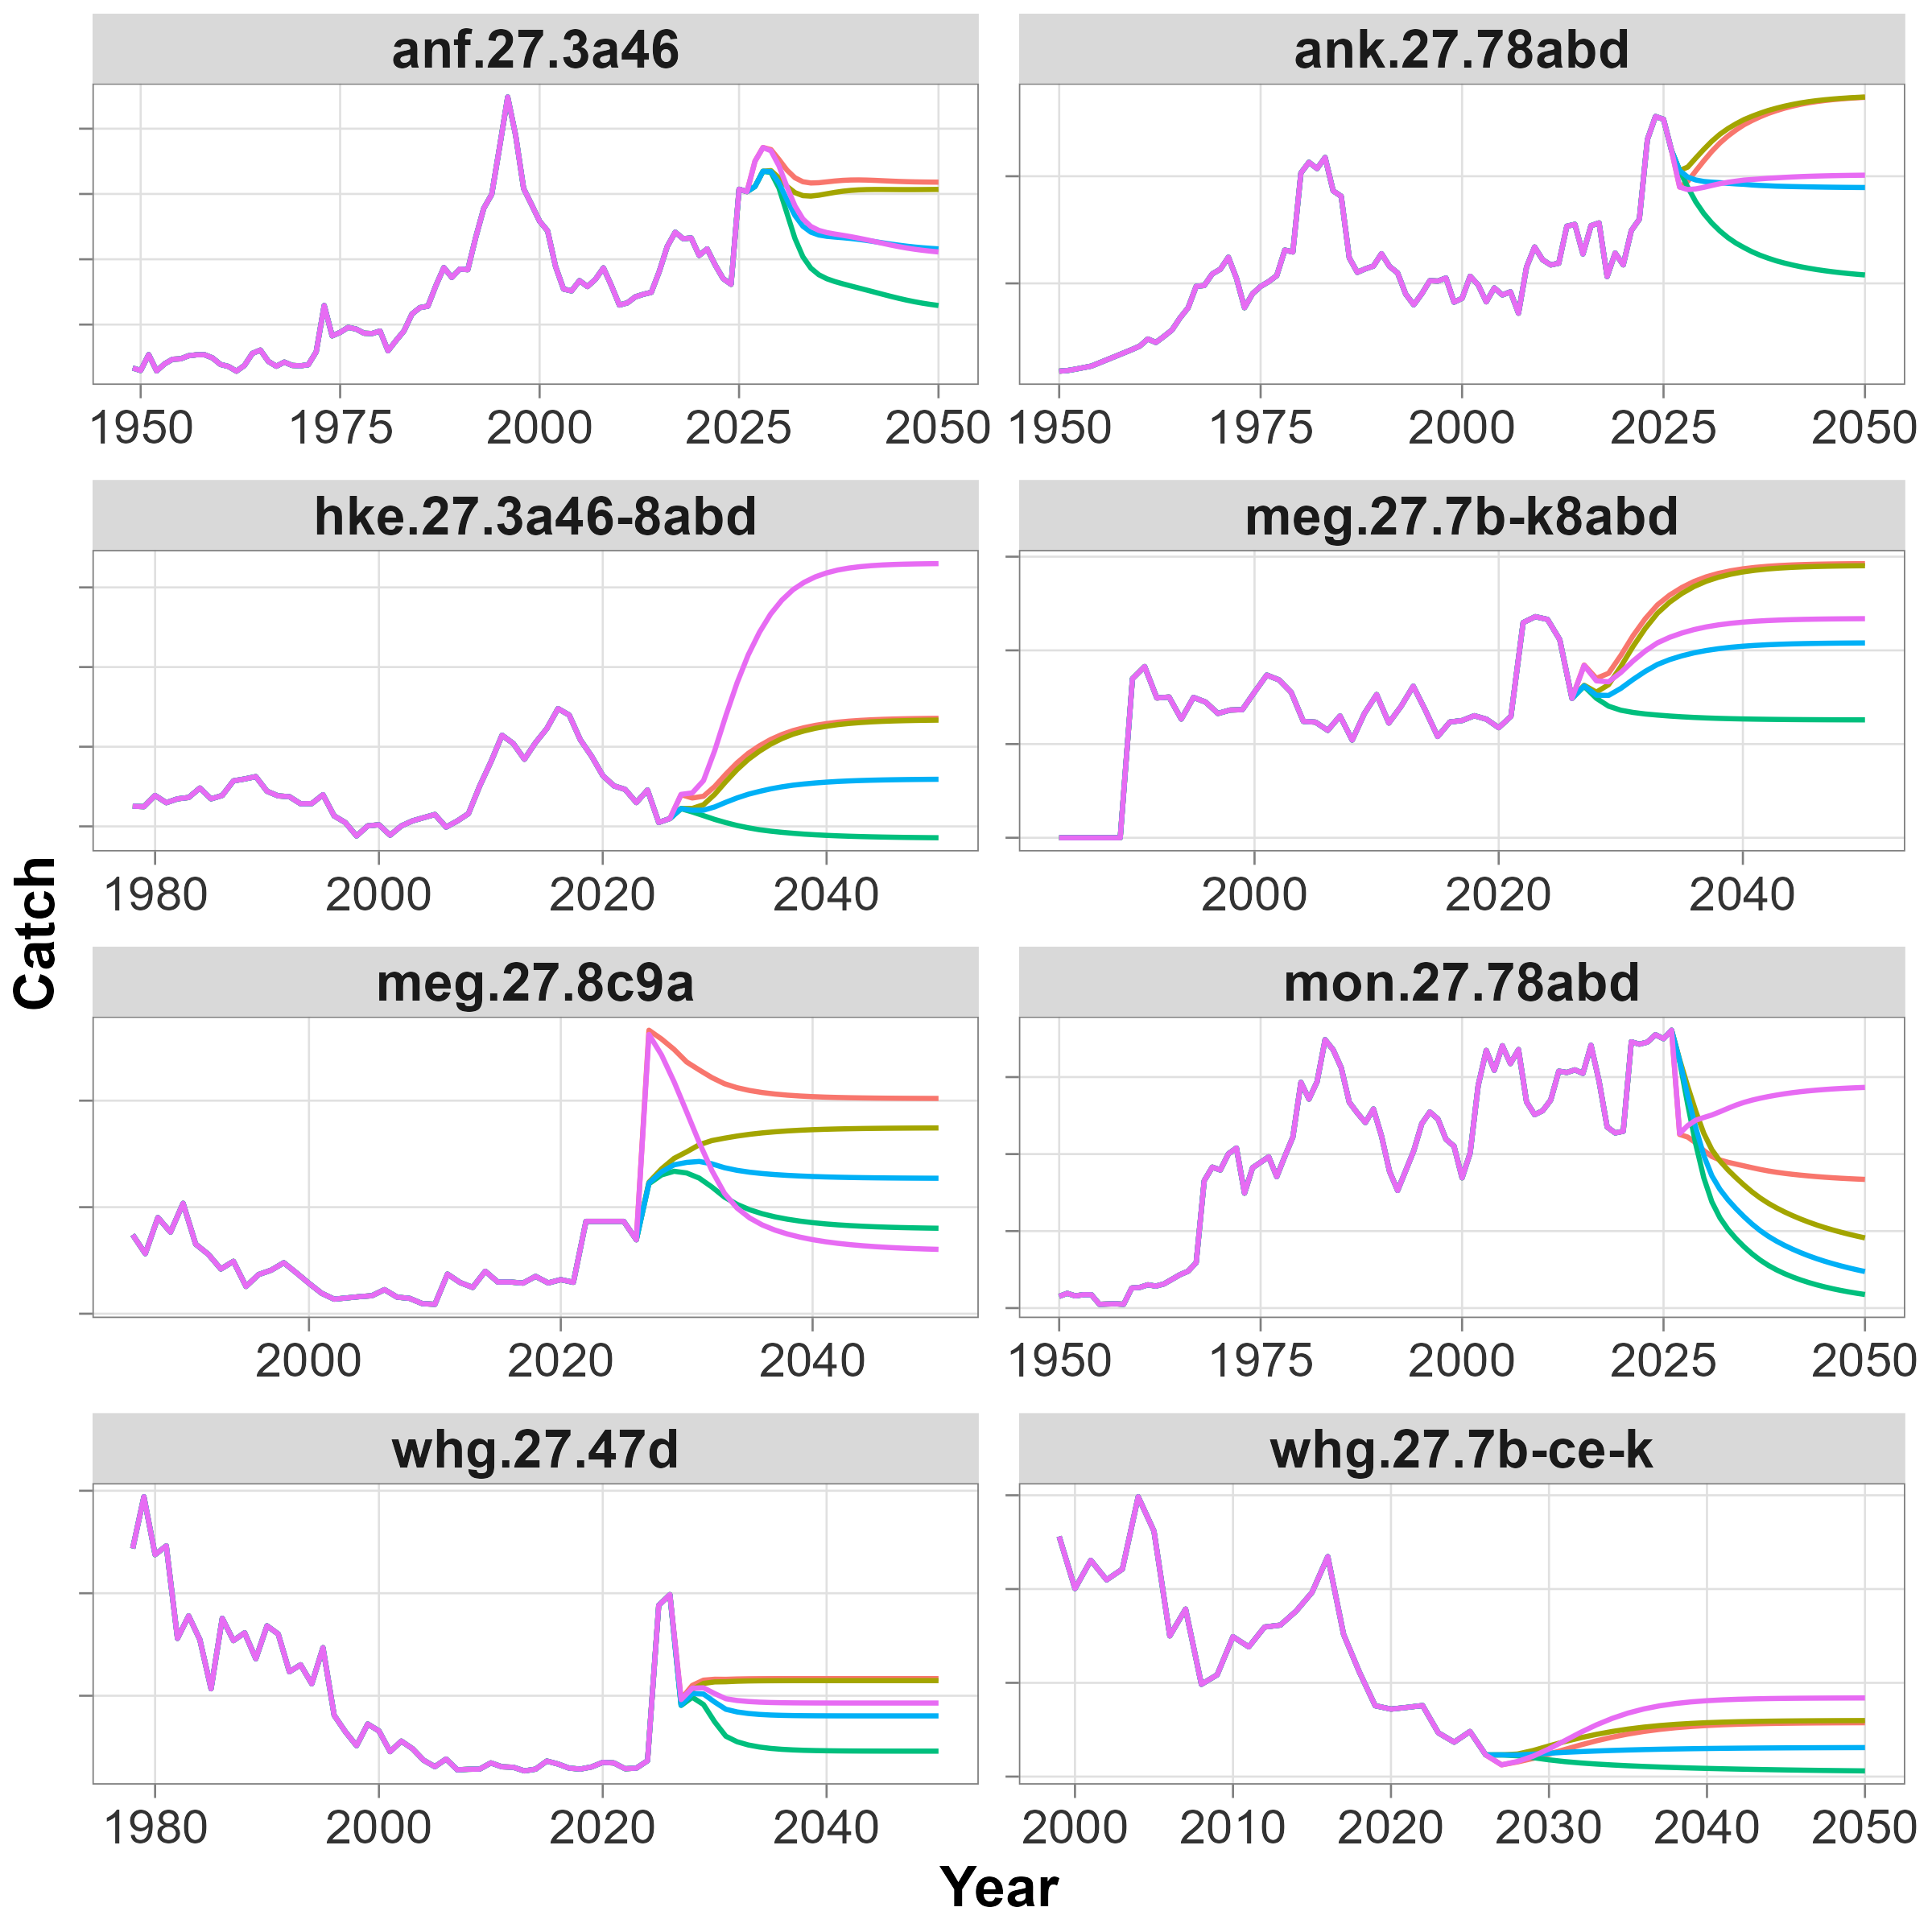
\includegraphics[width=\linewidth]{fig5.png}\\
      {\scriptsize Projected catch by scenario}
    \end{column}
  \end{columns}
\end{frame}

\begin{frame}{2. Scenarios --- \textit{Nephrops}}
  \begin{columns}[T]
    \begin{column}{0.46\textwidth}
      \footnotesize
      \begin{itemize}
        \item \textbf{\textit{Nephrops}}: functional units on harvest-rate OMs (JABBA / biodyn)
        \item Scenarios in harvest-rate space:
          \begin{itemize}
            \item Status-quo harvest; same harvest with process error $\times 0.75$ / $0.50$
            \item $F_{\mathrm{MSY}}$ harvest; $F_{\mathrm{MSY}}$ with autocorrelated process-error noise
          \end{itemize}
        \item Productivity shock enters via process error, not a recruitment residual
      \end{itemize}
    \end{column}
    \begin{column}{0.5\textwidth}
      \centering
      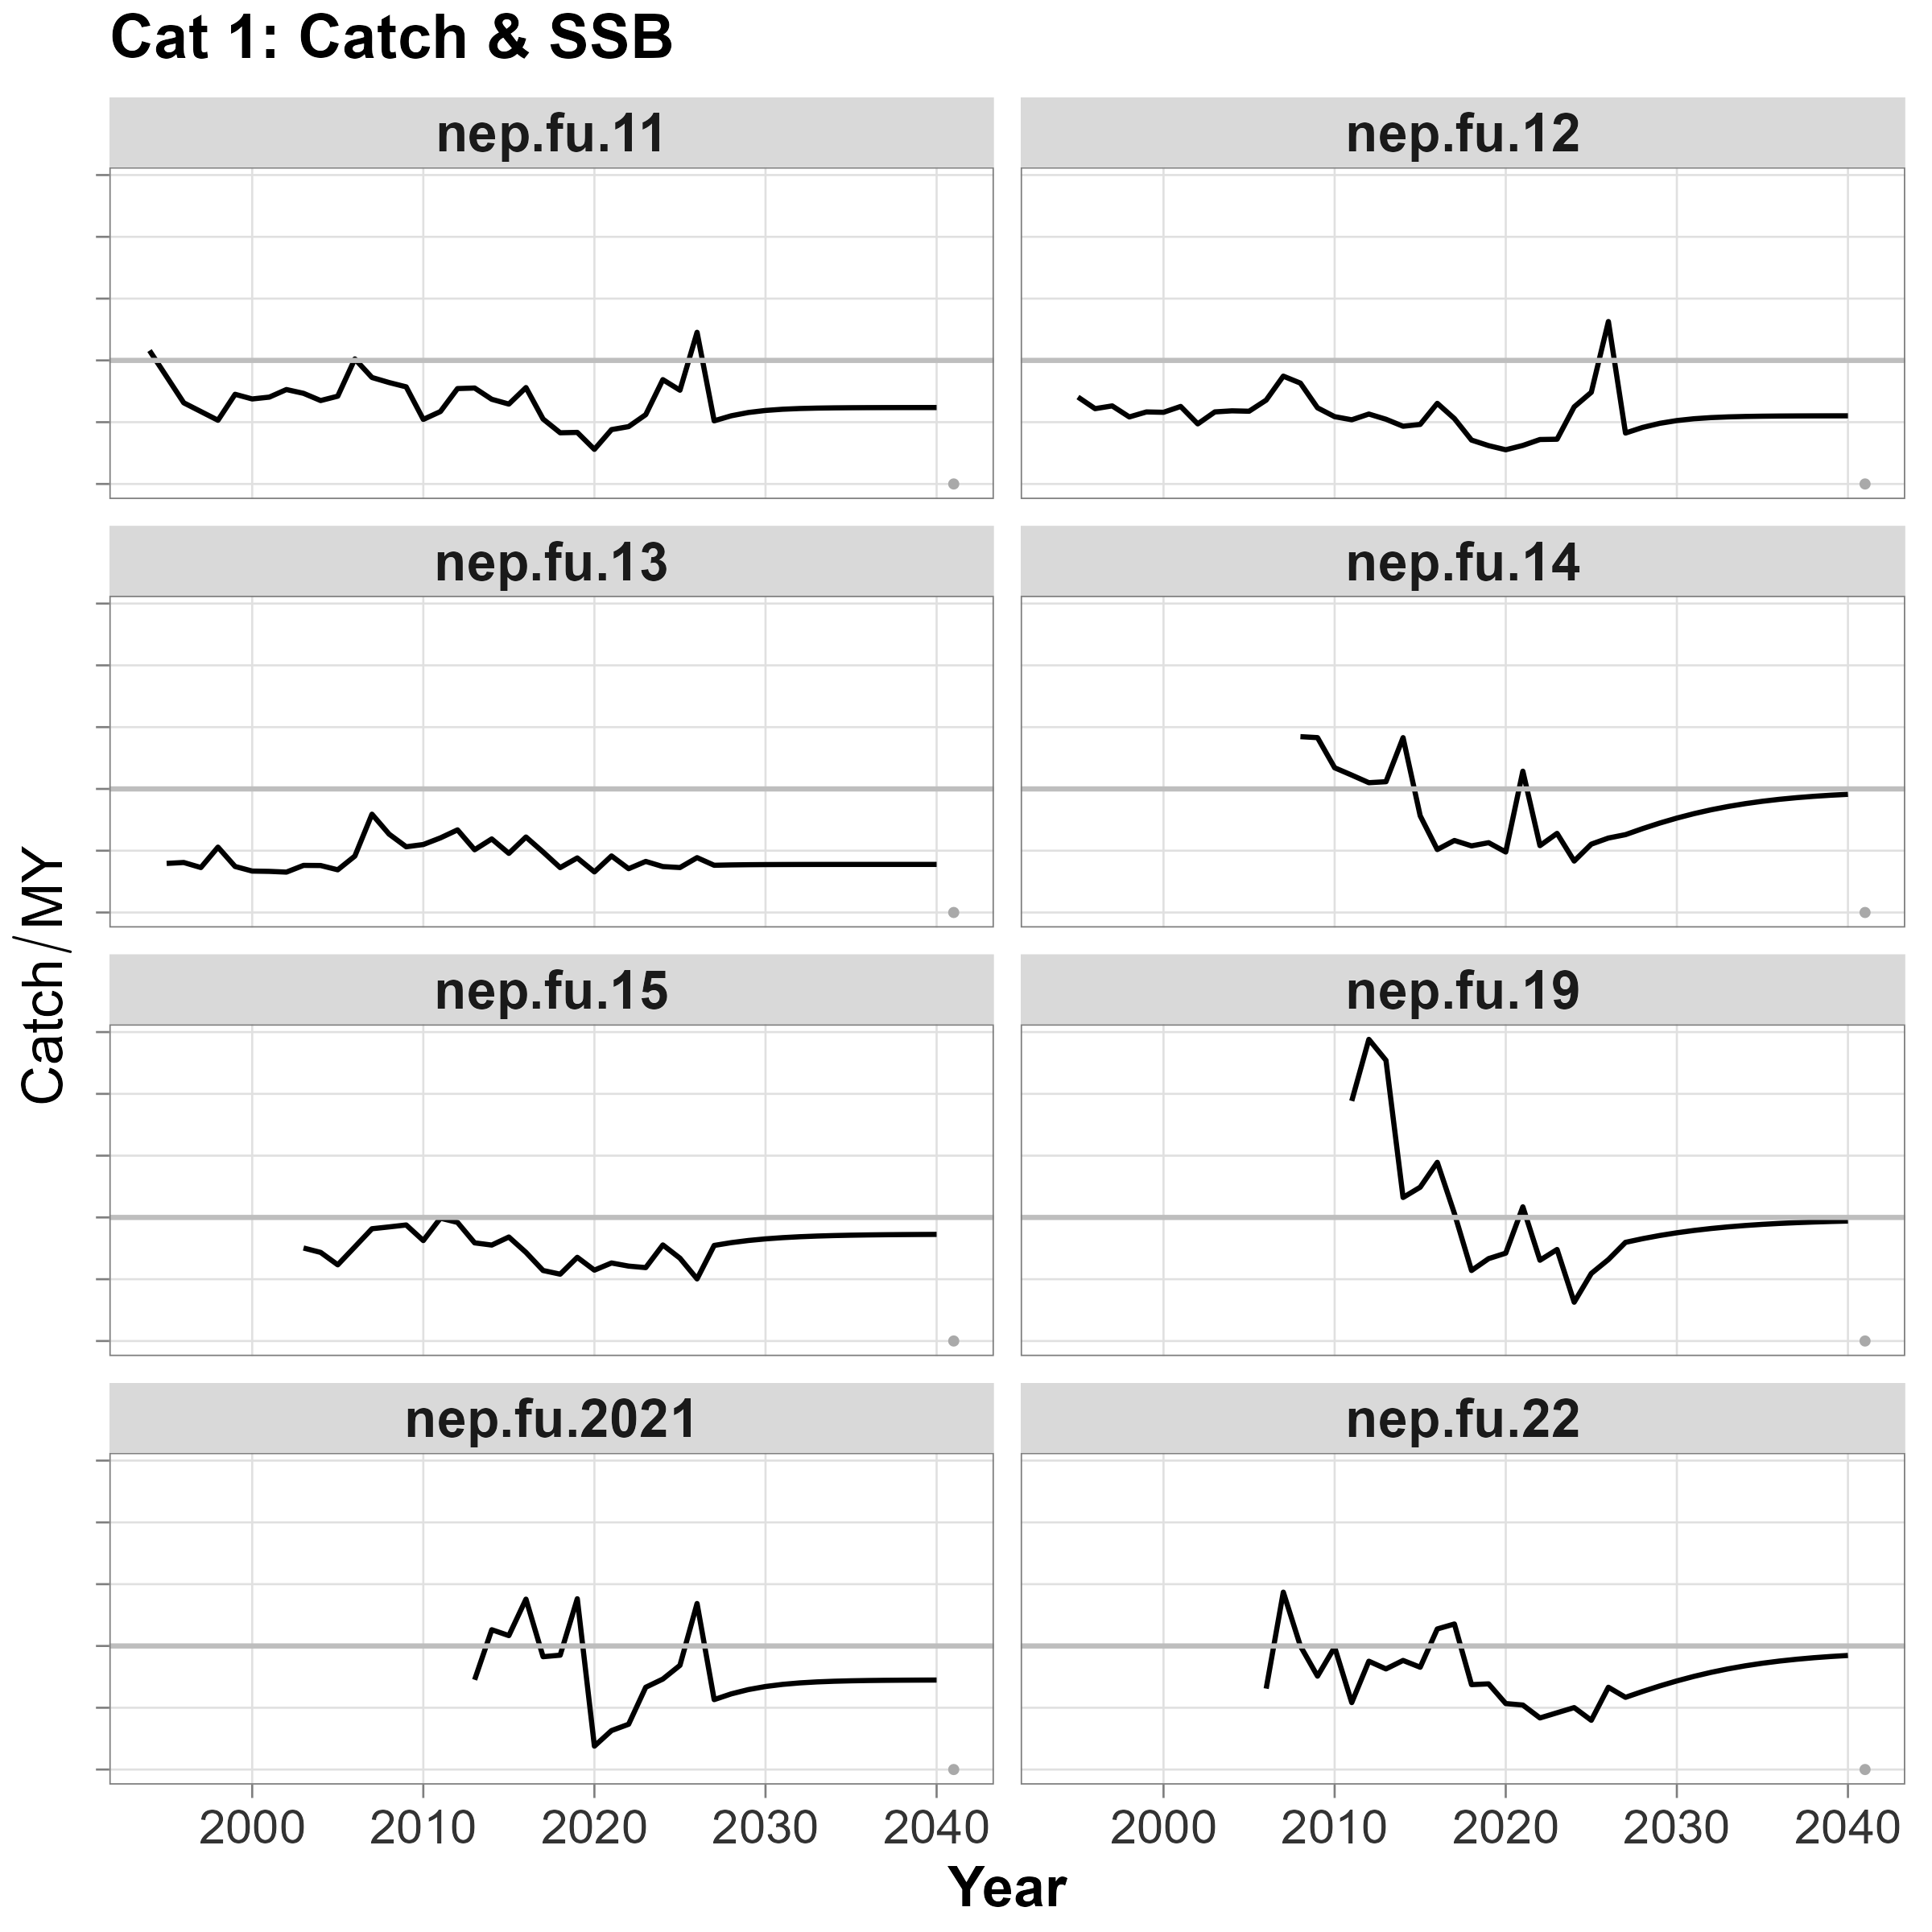
\includegraphics[width=\linewidth]{fig6.png}\\
      {\scriptsize Projected catch by scenario}
    \end{column}
  \end{columns}
\end{frame}

\begin{frame}{2. Scenarios --- mackerel: recruitment levels}
  \begin{columns}[T]
    \begin{column}{0.46\textwidth}
      \footnotesize
      \begin{itemize}
        \item \textbf{NEA mackerel} (\texttt{mac.27.nea}): worked example of industry-style ``what ifs''
        \item Fixed status-quo $F$; recruitment deviance scaled relative to the recent residual mean
          \begin{itemize}
            \item $\times 1$, $\times 0.75$, $\times 0.5$, $\times 0.25$
          \end{itemize}
        \item Asks: if fishing stays as now, how much does catch erode when productivity is poorer?
      \end{itemize}
    \end{column}
    \begin{column}{0.5\textwidth}
      \centering
      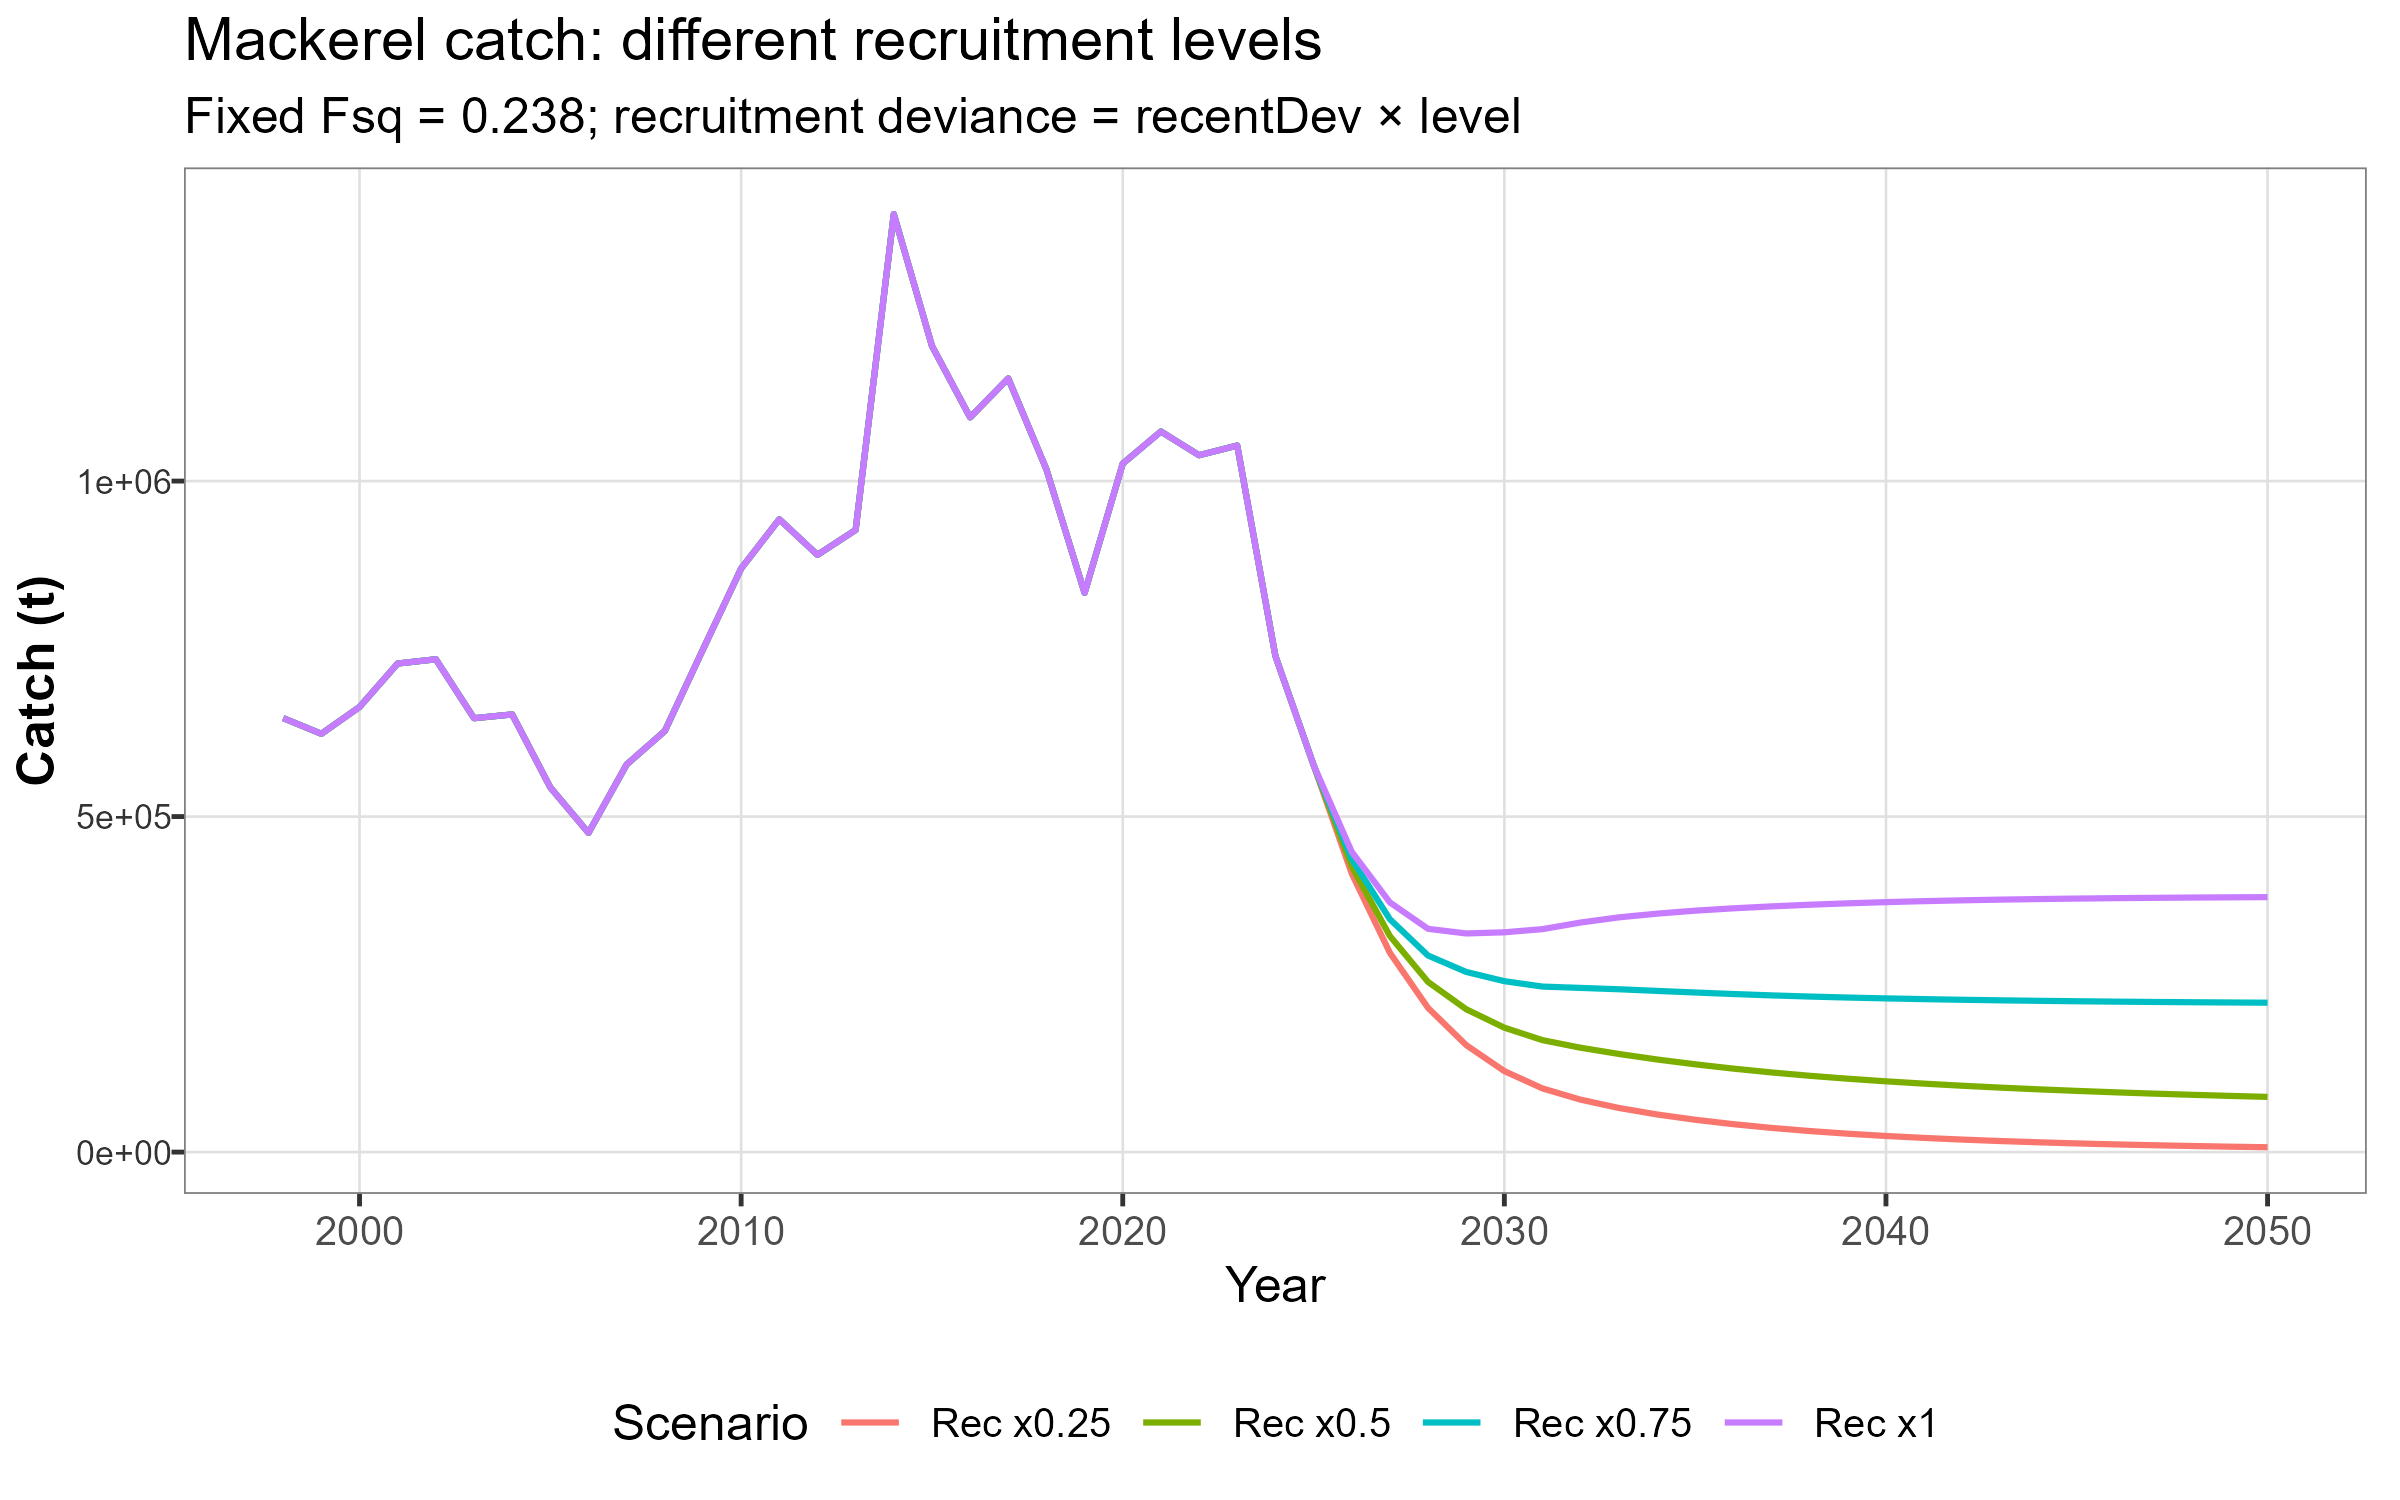
\includegraphics[width=\linewidth]{fig_mac_rec.png}\\
      {\scriptsize Catch under recruitment multipliers}
    \end{column}
  \end{columns}
\end{frame}

\begin{frame}{2. Scenarios --- mackerel: one-off $M$ shock}
  \begin{columns}[T]
    \begin{column}{0.46\textwidth}
      \footnotesize
      \begin{itemize}
        \item Same status-quo $F$ and baseline recruitment deviance
        \item \textbf{Shock}: natural mortality $\times 5$ for a single year (2035), then back to baseline $M$
        \item A pulse, not a trend --- the kind of flip a smooth forecast would miss
        \item Compare shocked path with the no-shock baseline
      \end{itemize}
    \end{column}
    \begin{column}{0.5\textwidth}
      \centering
      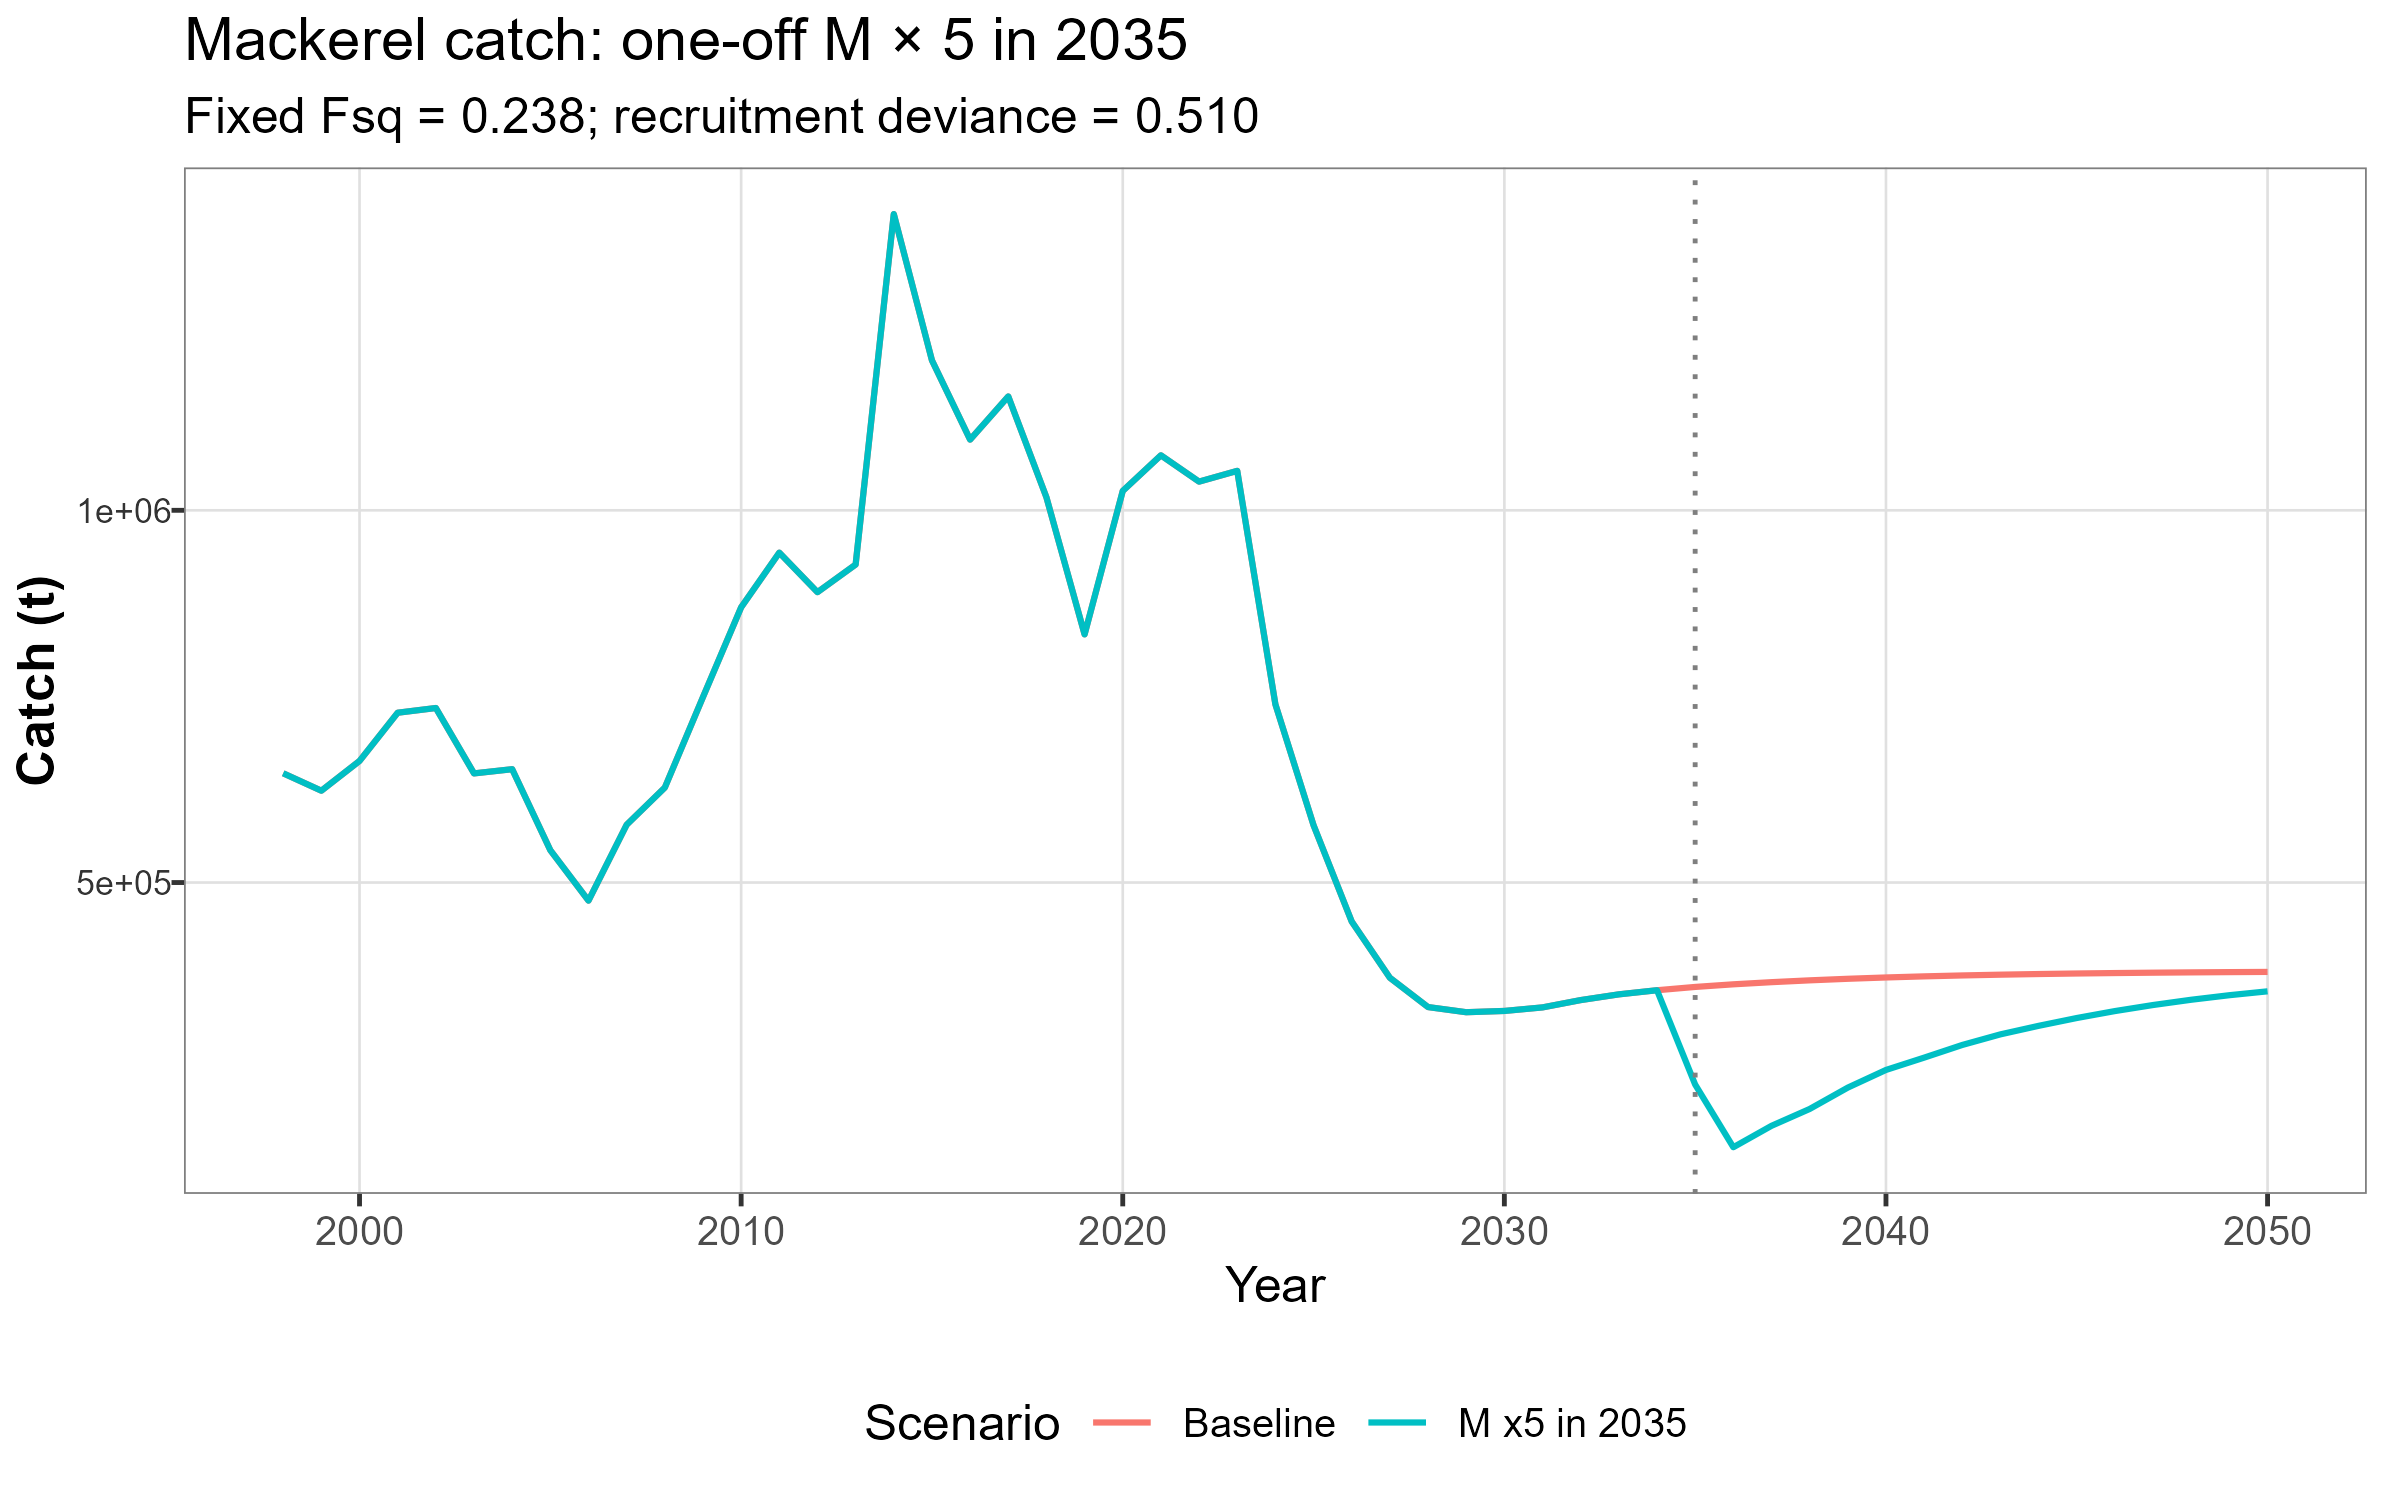
\includegraphics[width=\linewidth]{fig_mac_mshock.png}\\
      {\scriptsize Catch: baseline vs $M\times 5$ in 2035}
    \end{column}
  \end{columns}
\end{frame}

\begin{frame}{2. Scenarios --- mackerel: random recruitment}
  \begin{columns}[T]
    \begin{column}{0.46\textwidth}
      \footnotesize
      \begin{itemize}
        \item Year-to-year lognormal noise around the recent residual mean (sd from historical residuals)
        \item Fixed status-quo $F$; 50 iterations
        \item Ribbon = 5--95\% of catch paths; black line = one example iteration
        \item Shows the \emph{spread} resilience planning has to live with, not just a mean path
      \end{itemize}
    \end{column}
    \begin{column}{0.5\textwidth}
      \centering
      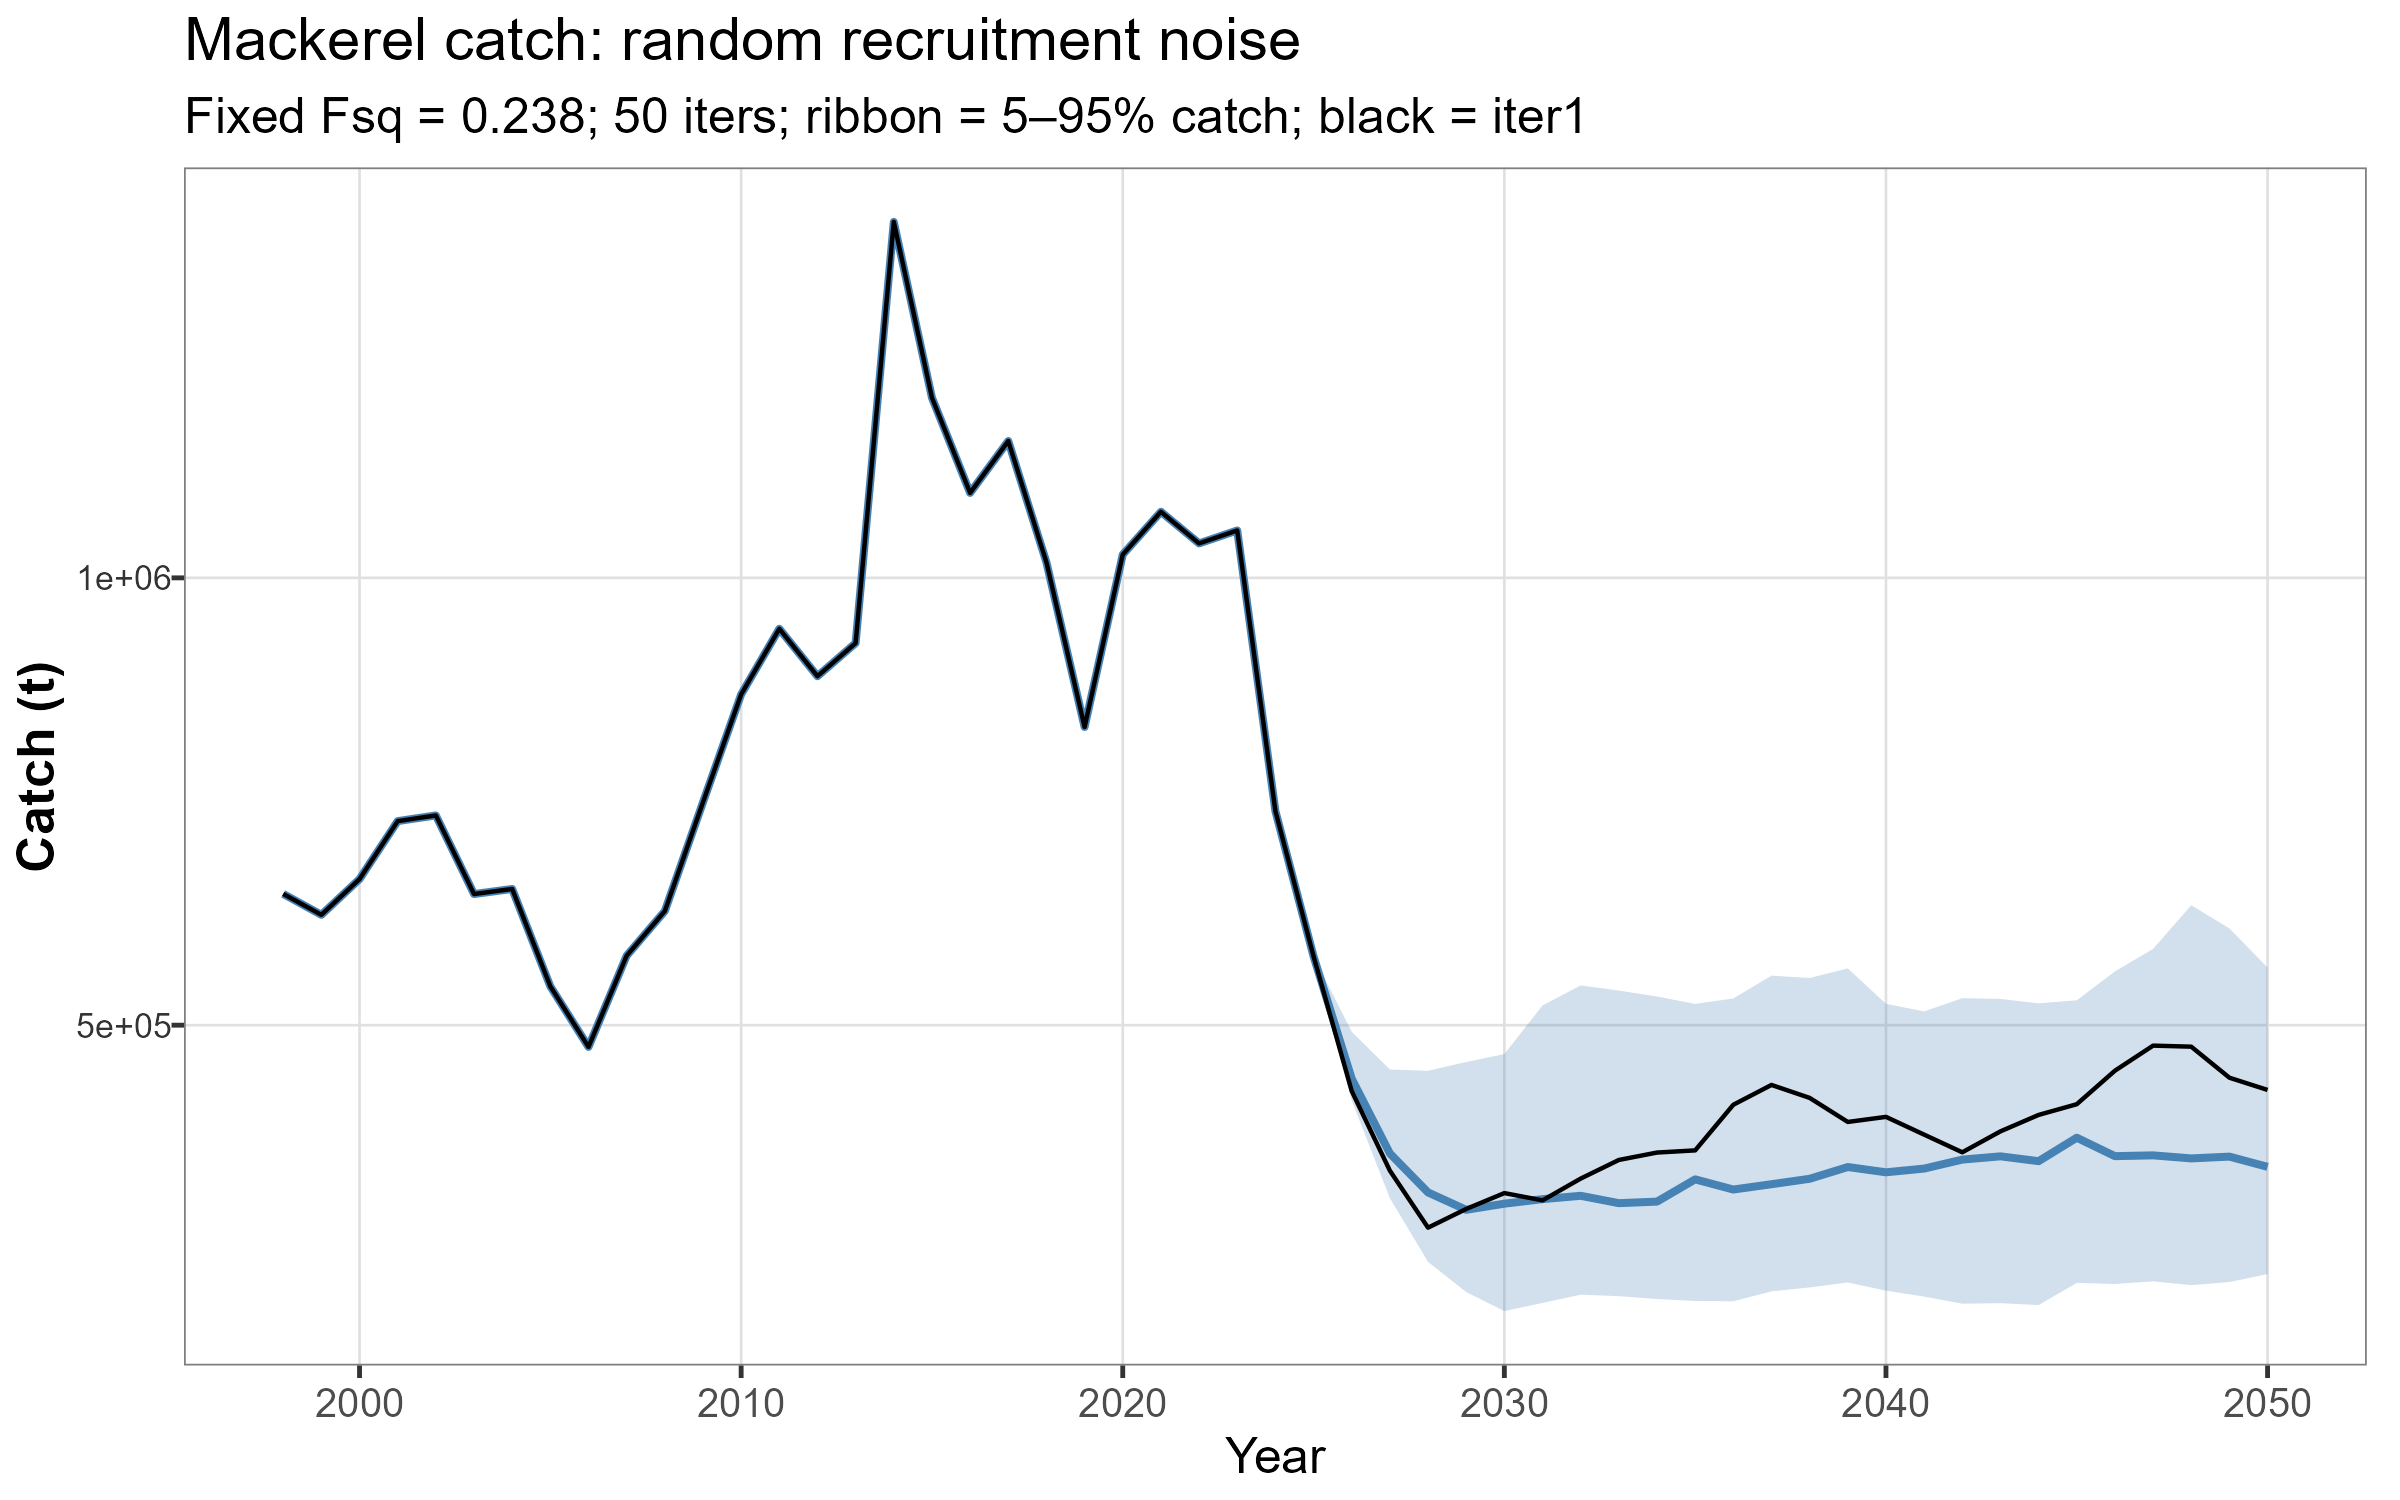
\includegraphics[width=\linewidth]{fig_mac_rand.png}\\
      {\scriptsize Stochastic catch: median, band, example path}
    \end{column}
  \end{columns}
\end{frame}

% ------------------------------------------------------------
\section{CREST}

\begin{frame}{3. CREST --- not an answering machine}
  \begin{columns}[T]
    \begin{column}{0.52\textwidth}
      \footnotesize
      \begin{itemize}
        \item \textbf{Industry formulates the question}: \textit{``what if this happens?''}
        \item That question becomes a scenario, tested to see if the fleet is
          \begin{itemize}
            \item resilient to it, or
            \item should be
          \end{itemize}
        \item \textbf{Capacity, Resilience and Economic Shock Transmission}: a fleet-segmented bio-economic model carrying a biological, regulatory or market shock through to landed value, effort and profitability by fleet segment
        \item Sits between a stock assessment (no population feedback) and a whole-economy model (no macro adjustment)
        \item Framed around \textbf{shocks or flips}, not trend extrapolation --- quota cuts, price collapses, regime changes a smooth trend would miss
      \end{itemize}
    \end{column}
    \begin{column}{0.44\textwidth}
      \centering
      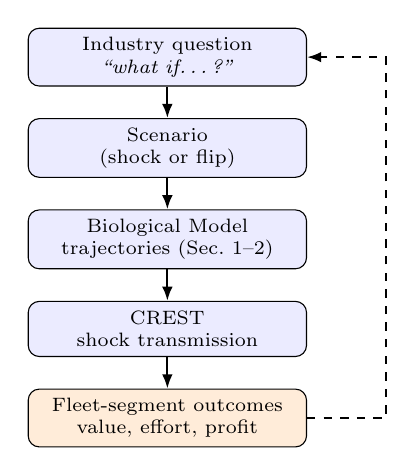
\begin{tikzpicture}[
          node distance=4mm and 4mm,
          box/.style={draw, rounded corners, fill=blue!8, align=center, minimum height=7mm, text width=3.3cm, font=\scriptsize},
          arr/.style={-{Latex[length=1.8mm]}, thick}
        ]
        \node[box] (q) {Industry question\\\emph{``what if\dots?''}};
        \node[box, below=of q] (s) {Scenario \\ (shock or flip)};
        \node[box, below=of s] (bm) {Biological Model \\ trajectories (Sec.\ 1--2)};
        \node[box, below=of bm] (crest) {CREST \\ shock transmission};
        \node[box, below=of crest, fill=orange!15] (out) {Fleet-segment outcomes \\ value, effort, profit};
        \draw[arr] (q) -- (s);
        \draw[arr] (s) -- (bm);
        \draw[arr] (bm) -- (crest);
        \draw[arr] (crest) -- (out);
        \draw[arr, dashed] (out.east) -- ++(1.0,0) |- (q.east);
      \end{tikzpicture}

      \vspace{2mm}

      \scriptsize Outcomes reframe the next question --- is the fleet resilient, or should it be?\par
    \end{column}
  \end{columns}
\end{frame}

% ------------------------------------------------------------
\section{Expert}

\begin{frame}{4. Expert --- eliciting the uncertainties that matter}
  \begin{columns}[T]
    \begin{column}{0.56\textwidth}
      \footnotesize
      \begin{itemize}
        \item Scoping \emph{which} shocks and flips are worth testing is a formal step: structured elicitation of expert and stakeholder judgement, not just an analyst's own list
        \item Precedent, Eastern Atlantic bluefin tuna (ICCAT/GBYP): 33 sources of uncertainty across 8 categories (reference points, recruitment, population structure, model, management, life history, environment, catch), scored for \emph{importance}, \emph{knowledge} and \emph{representation} (Leach et al., 2014)
        \item That prioritisation feeds CREST's scenario design --- which industry-posed ``what ifs'' are worth the modelling effort
        \item Economic risk is also a policy-response question: insurance and mutual-fund mechanisms have been proposed to mediate the revenue risk shocks create for fishers (Mumford et al., 2009)
      \end{itemize}
    \end{column}
    \begin{column}{0.38\textwidth}
      \footnotesize
      \centering
      \textbf{Elicitation dimensions}
      \begin{itemize}
        \item Importance --- impact on management objectives
        \item Knowledge --- scope to reduce via research
        \item Representation --- covered in the current assessment?
      \end{itemize}
      \vspace{2mm}
      \textbf{Response mechanism}
      \begin{itemize}
        \item Insurance / mutual funds to smooth revenue shocks, reward compliant, risk-reducing behaviour
      \end{itemize}
    \end{column}
  \end{columns}
\end{frame}

% ------------------------------------------------------------
\begin{frame}{References}
  \footnotesize
  \begin{itemize}
    \item Kell, L.T. (2026). \textit{Simulation of future TACs}, draft standalone chapter, BIM Resilience report.
    \item Mumford, J.D., Leach, A.W., Levontin, P., Kell, L.T. (2009). Insurance mechanisms to mediate economic risks in marine fisheries. \textit{ICES Journal of Marine Science}, 66(5), 950--959. \url{https://doi.org/10.1093/icesjms/fsp100}
    \item Leach, A.W., Levontin, P., Holt, J., Kell, L.T., Mumford, J.D. (2014). Identification and prioritization of uncertainties for management of Eastern Atlantic bluefin tuna (\textit{Thunnus thynnus}). \textit{Marine Policy}, 48, 84--92. \url{https://doi.org/10.1016/j.marpol.2014.03.010}
  \end{itemize}
\end{frame}

\end{document}
